%\graphicspath{Figures/detector}

\chapter{The \LHC and \CMS experiment}
\label{chap:detector}

\chapterquote{Insanity: doing the same thing over and over again and expecting different results.}
{Albert Einstein, 1879 –- 1955}

Probing the physics of the \ac{SM} and beyond at the~\TeV scale is only possible with the technologically unparalleled apparatus situated at the \ac{CERN}.
This chapter will introduce the hugely complex machinery of the \LHC, 
which provides proton-proton collisions at centre-of-mass energies in excess of $\sqrt{s}=7$~\TeV, 
and outline the main features of the \ac{CMS} experiment, of which the author is a member, 
with particular focus on those features relevant to the material presented in this thesis.
%exploited in the search for new physics using monojet events.
%
Section~\ref{sec:LHC} presents the main features of the \ac{LHC}, and Section~\ref{sec:CMS} provides an overview of the \ac{CMS} detector. Physics bject reconstruction is described in Section~\ref{sec:CMSreco} and the \ac{CMS} trigger system is discussed in Section~\ref{sec:CMStrig}. 

%%%%%%%%%%%%%%%%%%%%%%%%%%%%%%%%%%%%%%%%%%%%%%%%%%%%%%%%%%%%%%%%%%%%%%%%%%%%%%%%%%%%%%%%%%%%%%% 
%  _      _    _  _____ 
% | |    | |  | |/ ____|
% | |    | |__| | |     
% | |    |  __  | |     
% | |____| |  | | |____ 
% |______|_|  |_|\_____|
%                                                                  
%%%%%%%%%%%%%%%%%%%%%%%%%%%%%%%%%%%%%%%%%%%%%%%%%%%%%%%%%%%%%%%%%%%%%%%%%%%%%%%%%%%%%%%%%%%%%%%

\section{The \LHC}
\label{sec:LHC}
The \ac{LHC} is the world's largest and most energetic synchrotron particle collider. 
Housed in the tunnel built for the \ac{LEP} collider that operated during the 1990's at \ac{CERN}, 
the \ac{LHC} is a double ring circular collider 27~\km in circumference, 
and sits on the bedrock beneath the Franco-Swiss border, close to Geneva, Switzerland. 
It is designed for both proton-proton (pp) and heavy ion (PbPb) collisions at a centre of mass energy $\sqrt{s} = 14~\TeV$ and luminosity of \designLumi.


Currently the world's only operating collider able to study physics directly at the~\TeV scale, the \ac{LHC} consists of thousands of superconducting magnets which act to accelerate, bend and focus two beams of protons (or heavy ions) that circulate in opposite directions around the accelerator. 
%injector chain
A chain of accelerators, shown in Figure~\ref{fig:LHC} and culminating with the \ac{SPS}, inject bunches of approximately one hundred billion protons 25 or 50~\ns apart at $\sqrt{s} = 450~\GeV$ into the two beams of \ac{LHC}.
Oscillating electric fields provided by 1232 superconducting dipole magnets act to accelerate the beams up to the operating centre of mass energy, which for the data used in this thesis was $\sqrt{s} = 8$~\TeV, with bunch crossings every 50~\ns.
Once protons are accelerated to the operational $\sqrt{s}$, the \ac{LHC} acts as a storage ring, and collisions can occur.
%
Either side of four points around the \ac{LHC} ring, very high precision magnetic fields, provided by quadrupole and higher order multipole magnets, position and focus the beams such that each bunch has a diameter of 16~$\mu$m. 
The chance of a pp collision with large momentum transfer at the four interaction points around the LHC ring is thereby increased, and the number of such collisions per bunch crossing, termed \ac{PU} for the data used in this thesis was $\sim20$.

%picture
\begin{figure}[htbp]
  \begin{center}
  %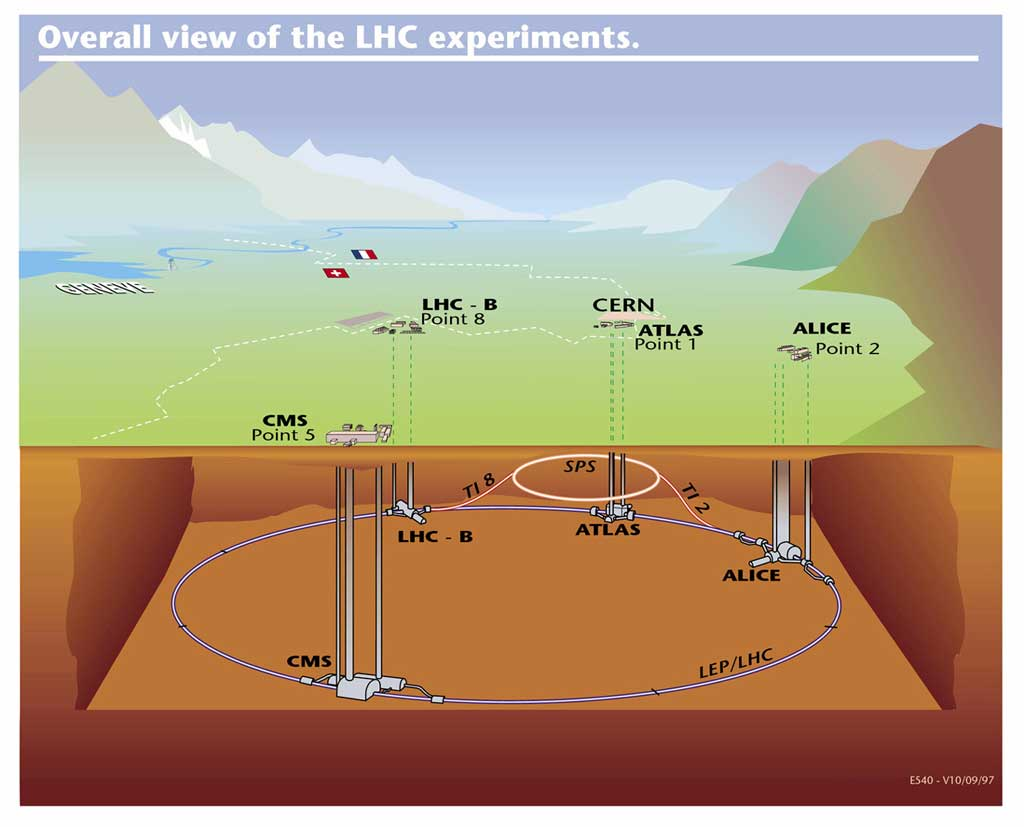
\includegraphics[width=0.8\textwidth]{Figures/detector/LHCdesign}
  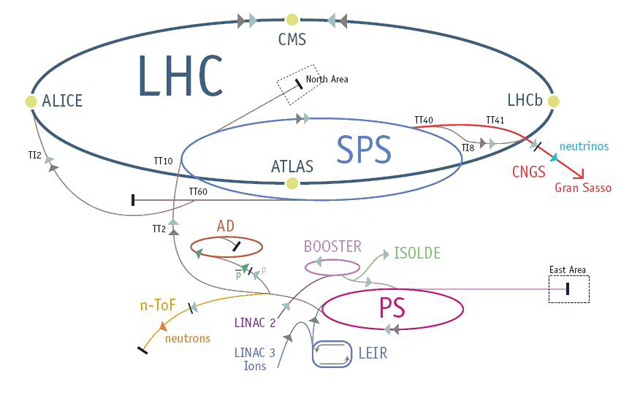
\includegraphics[width=0.8\textwidth]{Figures/detector/lhc}
  \caption{The ~\LHC accelerator ring, showing the locations of the four main experiments at the four collision points.
}
  \label{fig:LHC}
  \end{center}
\end{figure}

Interaction points are at the centre of four large particle detectors, shown in Figure~\ref{fig:LHC}:
\ac{ALICE}~\cite{Aamodt:2008zz}, 
\ac{ATLAS}~\cite{Aad:2008zzm}, 
\ac{CMS}~\cite{Chatrchyan:2008aa} and 
\ac{LHCb}~\cite{Alves:2008zz}.
They act to identify particles produced as a result of a pp or PbPb bunch crossing through a combination of tracking and calorimetry, in order to reconstruct and measure physical processes, to test currently accepted theories and search for new physics.

%running in Run 1

%%%%%%%%%%%%%%%%%%%%%%%%%%%%%%%%%%%%%%%%%%%%%%%%%%%%%%%%%%%%%%%%%%%%%%%%%%%%%%%%%%%%%%%%%%%%%%%
%   _____ __  __  _____ 
%  / ____|  \/  |/ ____|
% | |    | \  / | (___  
% | |    | |\/| |\___ \ 
% | |____| |  | |____) |
%  \_____|_|  |_|_____/ 
%                       
%%%%%%%%%%%%%%%%%%%%%%%%%%%%%%%%%%%%%%%%%%%%%%%%%%%%%%%%%%%%%%%%%%%%%%%%%%%%%%%%%%%%%%%%%%%%%%%

\section{The CMS Detector}
\label{sec:CMS}

The \ac{CMS} detector is a general purpose particle detector situated at Point 5 on the \ac{LHC} ring, designed to carry out many different measurements for various physics goals.
Close to 4$\pi$ solid angle reconstruction with 
efficient particle identification and reconstruction allows measurements of photons, muons, electrons, taus, hadronic showers and missing transverse momentum.
%It is therefore very well suited to the search for new physics, and direct production of \ac{SUSY}, in many different forms.
%Here, we focus on the search for new physics, particularly using the monojet final state.
%
A diagram of \ac{CMS} is shown in Figure~\ref{fig:CMS}. It is 21.6~\m long, 14.6~\m in diameter and weighs 12500~T. 
It consists of different sub-detectors, each of which measures a different particle or property, 
and is built around a central 12.5~m long 4~\T superconducting solenoid magnet and its iron return yoke.
%
\ac{CMS} consists of a barrel region, containing the solenoid, and endcaps to extend the forward and backward coverage.

%
The different sub-detectors are arranged in an onion structure.
%
Closest to the beam line is the silicon tracking system.
A very highly resolution pixel detector lies closest to the interaction region, followed by a granular strip detector.
Charged particle momenta measurements are made using the curvature of tracks in the uniform magnetic field provided by the solenoid, as well as measurements of displaced vertices and impact parameters which are essential for identifying heavy flavor decays. 
%
Energy measurements are provided by the calorimeters, which lie outside the tracker; the \ac{ECAL} and \ac{HCAL}. 
The highly granular \ac{ECAL} consists of 70,000 transparent lead tungstate crystals. 
%which cause electromagnetic showers and produce scintillation light 
As electrons and photons pass through, they cause electromagnetic showers in the crystals, which produce scintillation light.
% allowing position and energy measurements. 
%Scintillation light produced in the crystals is collected by photodetectors and used to infer the incident particle energy.
%
The sampling \ac{HCAL} consists of slabs of brass interleaved with plastic. 
Incident hadrons shower when passing through the absorber (brass), causing scintillation light to be produced in the active material (plastic) as the shower passes through.
%
Scintillation light produced in the crystals, or plastic, is collected by photodetectors and used to infer the incident particle energy and position.
%
The solenoid lies outside the \ac{HCAL} and provides a 3.8~\T axial magnetic field.
%
Embedded in the iron return yoke of the magnet sits the muon system. 
Three different types of muon detectors are used to identify muons and make momentum and charge measurements over a large kinematic range.
%
More information on the CMS detector can be found in Ref.~\cite{Chatrchyan:2008aa}.

%
% Crucial to the successful operation of \ac{CMS} is the trigger. 
% The pp interaction cross section is 100~\mb, while for example, the W boson production cross section is some 6 orders of magnitude less than this, and the rare physics processes that \ac{CMS} was built to search for, such as Higgs boson and \ac{SUSY} production, many times smaller still.
% The \ac{LHC} delivers an unprecedented high instantaneous luminosity so that such rare physics processes occur, but this also implies that the vast majority of the collisions result in `uninteresting' physics: namely \ac{QCD} processes.
% It would be impossible to record such high volumes of data that comes out of \ac{CMS}, some PB s$^{-1}$, and not useful to do so.
% Therefore, a very efficient method of recording those events that appear `interesting'  
% is necessary, to reduce the 40~\MHz event rate to a more manageable 100~\Hz.
% The two-tier trigger system fulfills this role, via a hardware based online \ac{L1} an software based offline \ac{HLT} and is described in Section~\ref{sec:CMStrig}.

%

%%%%%%%
% Inside the solenoid and closest to the beam line is the tracking system.
% In the uniform magnetic field provided by the solenoid, charged particles leave curved tracks 
% in the component silicon pixels and strips, under the influence of the Lorentz force.
% Momenta measurements are made by measuring the curvature of these tracks.
% %
% The next subsystems out are the calorimeters: the \ac{ECAL} and \ac{HCAL}. 
% Consisting of absorber materials which cause electromagnetic and hadron showers, they totally absorb a particle, prompting scintillation light proportional to its energy in the active material. 
% An energy measurement is made by measuring the scintillation light and inferring the energy of the incident particle.
% %
% Finally, embedded in the return yoke of the magnet sit the muon systems. 
% Muons are relatively long lived, heavier and therefore more penetrating than other particles,
% so require detectors further away from the interaction point. 
% Three different types of muon detectors, interleaved with the steel return yoke of the solenoid, are used to identify muons and make momentum and charge measurements over a large kinematic range.
% %
% More information on the CMS detector can be found in Ref.~\cite{Chatrchyan:2008aa}.

%picture
\begin{figure}[htbp]
  \begin{center}
  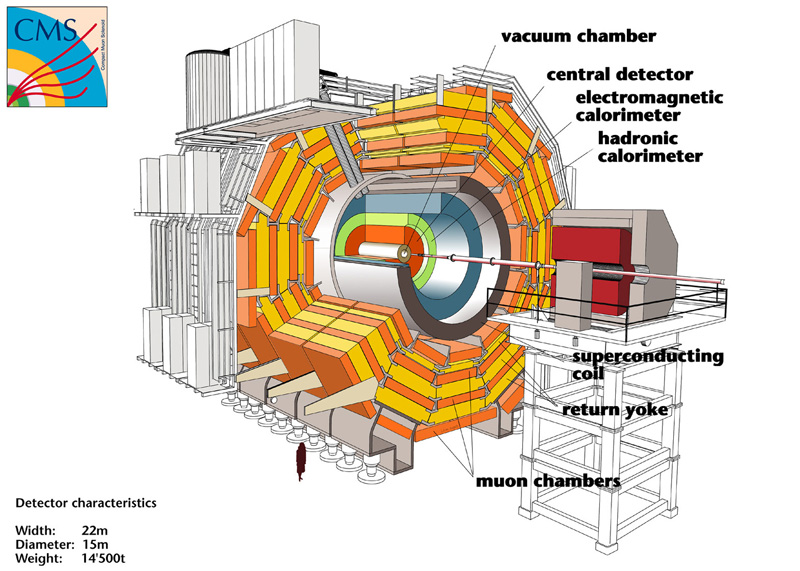
\includegraphics[width=0.8\textwidth]{Figures/detector/CMSlabelled}
  \caption{The \ac{CMS} detector, with the main subsystems labelled.
}
  \label{fig:CMS}
  \end{center}
\end{figure}

%coordinate system
\ac{CMS} uses a right-handed coordinate system: the $x$-axis points south towards the centre of the \ac{LHC} ring, the $y$-axis points vertically upwards and the $z$-axis is in the direction of the beam, where positive $z$ is to the West.
More natural is the coordinate system defined in terms of $r$, $\phi$ and $\theta$.
The azimuthal angle $\phi$ is measured from the $x$-axis in the $xy$ plane, where the radial component is denoted $r$. The polar angle $\theta$ is defined in the $rz$ plane, and the pseudorapity 
\begin{equation}
\eta = - \ln \tan (\theta /2).
\end{equation}
Convention is that the position of a particle is described in terms of $\eta$ and $\phi$, where $\eta = 0$ is along the $y$-axis and $\eta = \infty $ is along the beam direction; and $-\pi < \phi < \pi$. The distance between particles is commonly described in terms of the variable $\Delta R = \sqrt{\Delta\phi^2+\Delta\eta^2}$.

The \ac{LHC} is a hadron collider, and as such, collides non-fundamental particles. 
Inelastic collisions with large momentum transfer can occur between component quarks and gluons, however in a single bunch crossing there will also be many low energy, elastic, soft scatters, 
as well as the remnant part of any protons that have had a hard collision. 
As a result, the forward and backward directions are highly populated environments and therefore difficult to instrument due to high occupancy and radiation damage. 
\ac{CMS} has endcaps to extend the detector coverage at high $\eta$, however it is not possible to reconstruct the momentum of a single interaction in the direction of the beam.   
Additionally, interesting physics is a result of a hard collision, where energy is available for the creation of new particles. It can be characterized by the amount of energy in the transverse ($xy$) plane.
For these reasons, particle energy and momenta are described only in the transverse plane, where conservation laws can be applied.
By conserving energy and momentum in the transverse plane, any imbalance can be assigned to a particle leaving the detector without any trace; for example from a neutrino, or, from new physics processes such as \ac{DM} production
A nearly hermetic detector (with close to 4\pi coverage in solid angle) allow excellent particle reconstruction and measurements of missing transverse energy, the `tell-tale' sign of new physics, and make \ac{CMS} perfectly suited to searching for physics beyond the \ac{SM}.

%%%%%%%%%%%%%%%%%%%%%%%%%%%%%%%%%%%%%%%%%%%%%%%%%%%%%%%%%%%%%%%%%%%%%%%%

\subsection{The Tracking System}
The tracker is designed for precise and efficient measurement of charged particle trajectories (and therefore position and momentum) as they emerge from the interaction point.
Additionally, reconstruction of any secondary vertices is crucial for identifying heavy flavor decays such as jets that originate from b-quarks.

The \ac{LHC} provides bunch crossings every 25 or 50~\ns, resulting in $\sim$ 20 pp interactions, giving rise to of order 1000 particles. 
All of these traverse the tracker. 
The granularity of the tracker must be such that one can determine which of the $\sim$ 20 pp vertices each of the particles come from, 
and the electronics fast enough that the information is sent on in time for the next bunch crossing to arrive.
With such high particle fluxes, the tracker is also subject to a huge amount of radiation damage.
These conditions must be dealt with using the least amount of material possible in order to limit multiple scattering, photon conversion, bremsstrahlung and nuclear interactions.
To meet such criteria, and to have an estimated lifetime of 10 years, the tracker is constructed entirely from silicon.

The tracker consists of an all silicon pixel and strip detector.
Measuring 5.8~\m in length and 2.5~\m in diameter, with a total active area of 200~\msq, it surrounds the interaction region.
%pixel
The pixel detector has three layers in the barrel, at radii of 4.4~\cm, 7.3~\cm and 10.2~\cm. In the endcaps, there are two disks at distances $z=\pm 34.5, \pm 46.5~\cm$.
%strip
The strip detector has a length of 5.8~\m and a diameter of 2.4~\m, and is composed of four subsystems: the \ac{TIB}, \ac{TOB}, \ac{TID} and \ac{TEC}. The \ac{CMS} tracker geometry is shown in Figure~\ref{fig:CMStracker}.

%picture
\begin{figure}[htbp]
  \begin{center}
  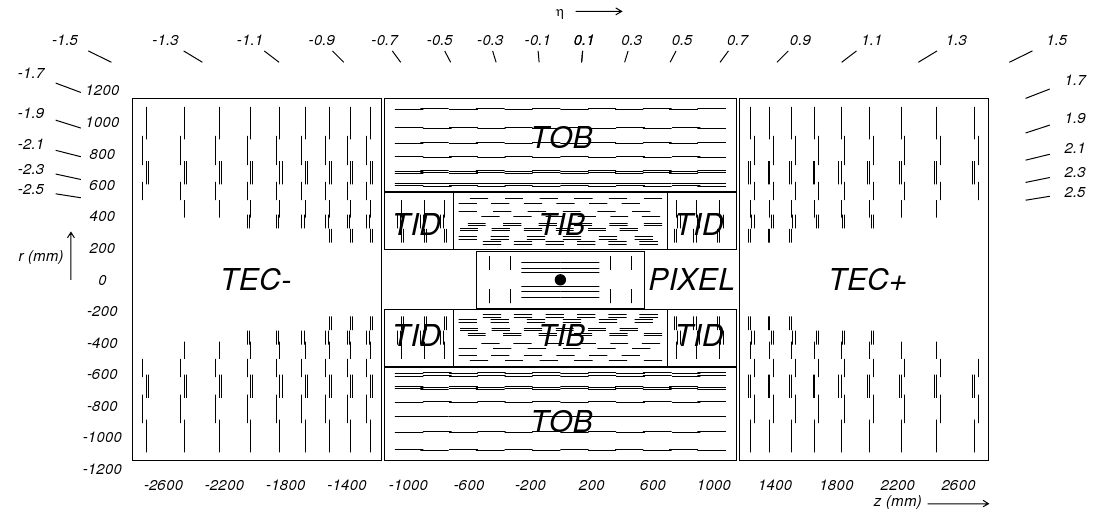
\includegraphics[width=0.9\textwidth]{Figures/detector/fig_cmstracker}
  \caption{The \ac{CMS} tracker, shown in the $rz$ plane. The pixel detector is shown at the centre of the tracker, closest to the interaction region (shown by the black dot), and the strip detector surrounds it. The different subsystems of the strip detector are shown. Taken from Ref.~~\cite{Chatrchyan:2008aa}.
}
  \label{fig:CMStracker}
  \end{center}
\end{figure}


%The resolution of a track is described in terms of five parameters
The energy resolution of the tracker is shown in Figure~\ref{fig:CMStrackerRes}, 
for samples of single muons with \pt of 1, 10 and 100~\GeV. 
For a 100\GeV muon, the resolution is 1-2\% up to $|\eta| = 1.6$. 
Lower momentum objects have a better energy resolution as their tracks have increased curvature.

%picture
\begin{figure}[htbp]
  \begin{center}
  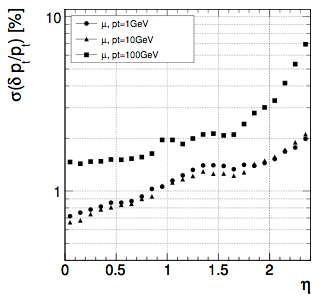
\includegraphics[width=0.3\textwidth]{Figures/detector/cmstrackerRes}
  \caption{The energy resolution as a function of $|\eta|$ for \ac{CMS} tracker, shown for single muons with \pt = 1, 10 and 100~\GeV. 
}
  \label{fig:CMStrackerRes}
  \end{center}
\end{figure}
%%%%%%%%%%%%%%%%%%%%%%%%%%%%%%%%%%%%%%%%%%%%%%%%%%%%%%%%%%%%%%%%%%%%%


\subsection{The Electromagnetic Calorimeter}
High resolution photon and electron position and energy measurements are provided by the lead tungstate (PbWO$_{4}$) crystal \ac{ECAL}, which covers pseudorapidty up to $|\eta|<3$.
It is made up of the \ac{EB}, covering the range $0<|\eta|<1.479$,
and the \ac{EE}, covering the range $1.479<|\eta|<3$.

Both fast response times (80\% of scintillation light is emitted in 25~\ns) and radiation hardness are required from the \ac{ECAL}, motivating the choice of material.
In addition, it is very dense (8.28~g$\cm^{-1}$), has a short radiation length ($X_{0} = 0.89~\cm$), and small Moli\`{e}re radius (2.2~\cm), making it well suited to a compact, fine granularity calorimeter.
Arranged in a quasi-projective geometry, 61,200 crystals in the barrel and 7,324 crystals in the endcaps are tapered in shape and angled at 3\deg to ensure that particle trajectories avoid cracks between them.
Barrel crystals have a front face of $22 \times 22$~mm$^{2}$ and a length of 23~\cm, corresponding to 25.8~$X_{0}$. 
Endcap crystals have a front face of $28.6 \times 28.6$~mm$^{2}$ and length corresponding to 24.7~$X_{0}$.
Electromagnetic showers are therefore expected to be contained within one crystal length, so only a single layer of crystals is needed. 
A preshower detector is place in front of the endcaps, with a thickness of $3X_{0}$, in the range $1.653<|\eta|<2.6$, in order to distinguish between single photons and photon pairs resulting from neutral pion decay. 
The \ac{ECAL} geometry is shown in Figure~\ref{fig:CMSecal}.

%picture
\begin{figure}[htbp]
  \begin{center}
  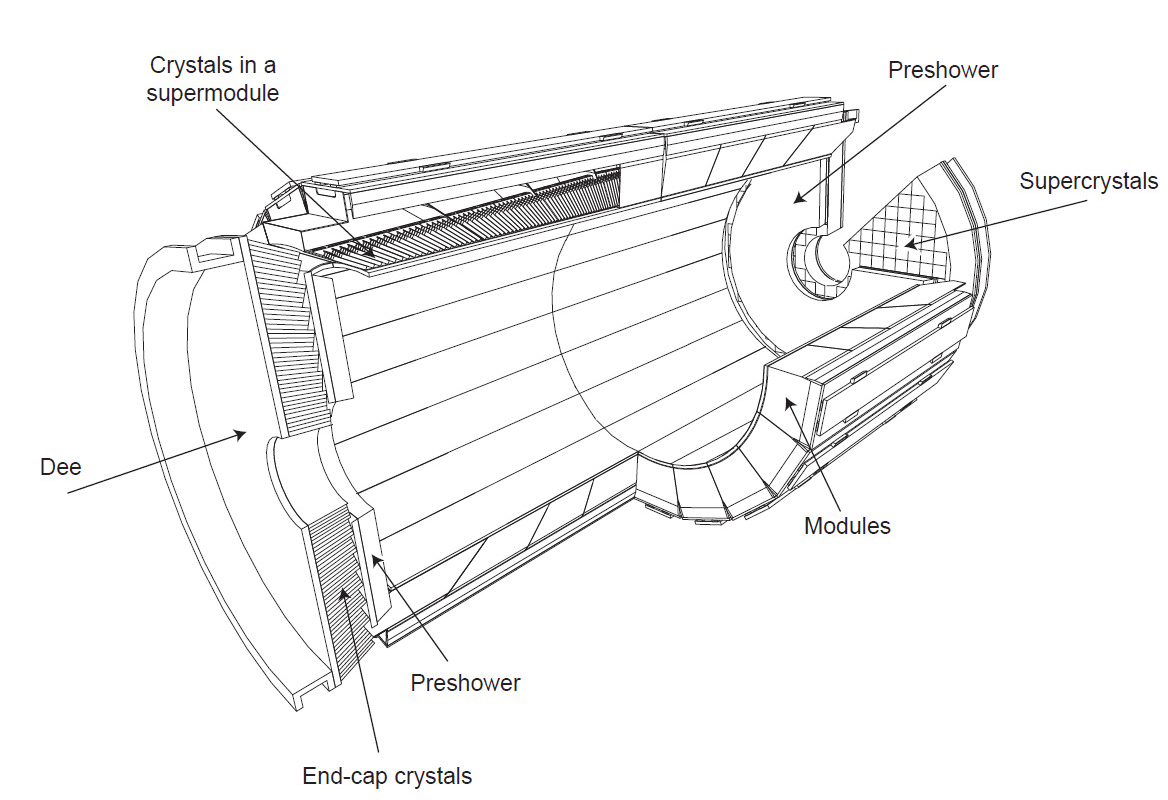
\includegraphics[width=0.7\textwidth]{Figures/detector/cmsECAL}
  \caption{Geometric view of the \ac{CMS} \ac{ECAL}. Barrel crystals are arranged in modules and supermodules, and endcap crystals arranged in supercrystals. Also shown is the preshower detector.
}
  \label{fig:CMSecal}
  \end{center}
\end{figure}

The very dense material PbWO$_{4}$ causes incident photons and electrons to shower. 
Resulting pair produced electrons and positrons, and radiated photons, cause scintillation light in the transparent, polished crystals. 
The amount of light produced is proportional to the incident particle energy, and is collected by an \ac{APD} on the end of each crystal in the barrel, and a \ac{VPT} in the endcaps. \textcolor{red}{[check if use these acronyms again]}
These photodetectors also have to be radiation hard and operate successfully in the 3.8~\T magnetic field, while providing significant amplification to signal.
Both the crystal and photodetector performance has a strong temperature dependence, so the \ac{ECAL} is kept at a constant temperature of 18\deg via a water cooling system, and is stable to $\pm0.05~\deg$C.

%energy resolution
The energy resolution of the \ac{ECAL} can be parametrised using the following equation:
\begin{equation}
\left(\frac{\sigma}{E}\right)^{2} = \left(\frac{S}{\sqrt{E}}\right)^{2} + \left(\frac{N}{E}\right)^{2} + C^{2},
\end{equation}
%laser calibration
where $S$ is due to stochastic scattering, $N$ is due to noise and $C$ is the constant term. Measurements in test beam are shown in Figure~\ref{fig:CMSecalRes}, where the terms were found to be: $S = 2.8\%$, $N=0.12~\GeV$ and $C = 0.30\%$. 

\begin{figure}
  \begin{center}
  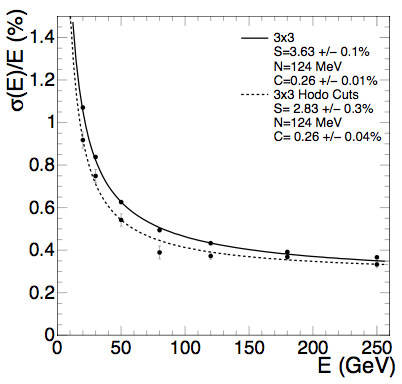
\includegraphics[width=0.5\textwidth]{Figures/detector/EcalRes.png}
  \caption{The energy resolution of an \ac{ECAL} supercrystal, measured in a test beam. The lower set of points along the dashed line correspond to the energy measured in an array of 3$\times$3 crystals, where events fall within a 4$\times$4~\mm region in the central crystal. 
}
  \label{fig:CMSecalRes}
  \end{center}
\end{figure}

%%%%%%%%%%%%%%%%%%%%%%%%%%%%%%%%%%%%%%%%%%%%%%%%%%%%%%%%%%%%%%%%%%%%%


\subsection{The Hadronic Calorimeter}
The \ac{HCAL} provides complementary energy measurements of hadronic showers, crucial for measuring jets and missing transverse energy.
It is a sampling brass calorimeter, built from alternating layers of large, absorbing brass plates, interleaved with scintillating plastic tiles arranged in trays. 
Sitting within the bore of the solenoid, the \ac{HB} covers pseudorapidity $|\eta|<1.3$,
and the \ac{HE} on each side enclose $1.3<|\eta|<3$.
To attain a most hermetic detector, there is also a \ac{HF}, which extends coverage right up to $|\eta|<5.2$.

The quality of the \ac{HCAL}'s measurements is dictated by the fraction of the hadronic shower that passes through the scintillator; the plastic must be thick enough to catch the majority of the shower.
This demand for radial extension is at odds with the location of the \ac{HCAL}, from the outer edge of the \ac{ECAL} at $r=1.77~\m$, and the inner edge of the solenoid at $r=2.95~\m$.
Providing a compromise, an outer hadronic calorimeter, \ac{HO}, is placed outside of the vacuum tank of the magnet and supplements the \ac{HB}.
Using the solenoid coil as absorber material, it can identify late starting showers, providing sufficient containment for 11.8 interaction lengths.% ($\lambda_{L}$).
Five rings of \ac{HO} are arranged along the $z$-axis of the detector, where the central ring at $\eta=0$ has two layers at $r=3.82~\m$ and $4.07~\m$, and the rest have a single layer at $r=4.07~\m$. 
Figure~\ref{fig:CMShcal} shows the geometry of the \ac{HCAL}.

%picture
\begin{figure}[htbp]
  \begin{center}
  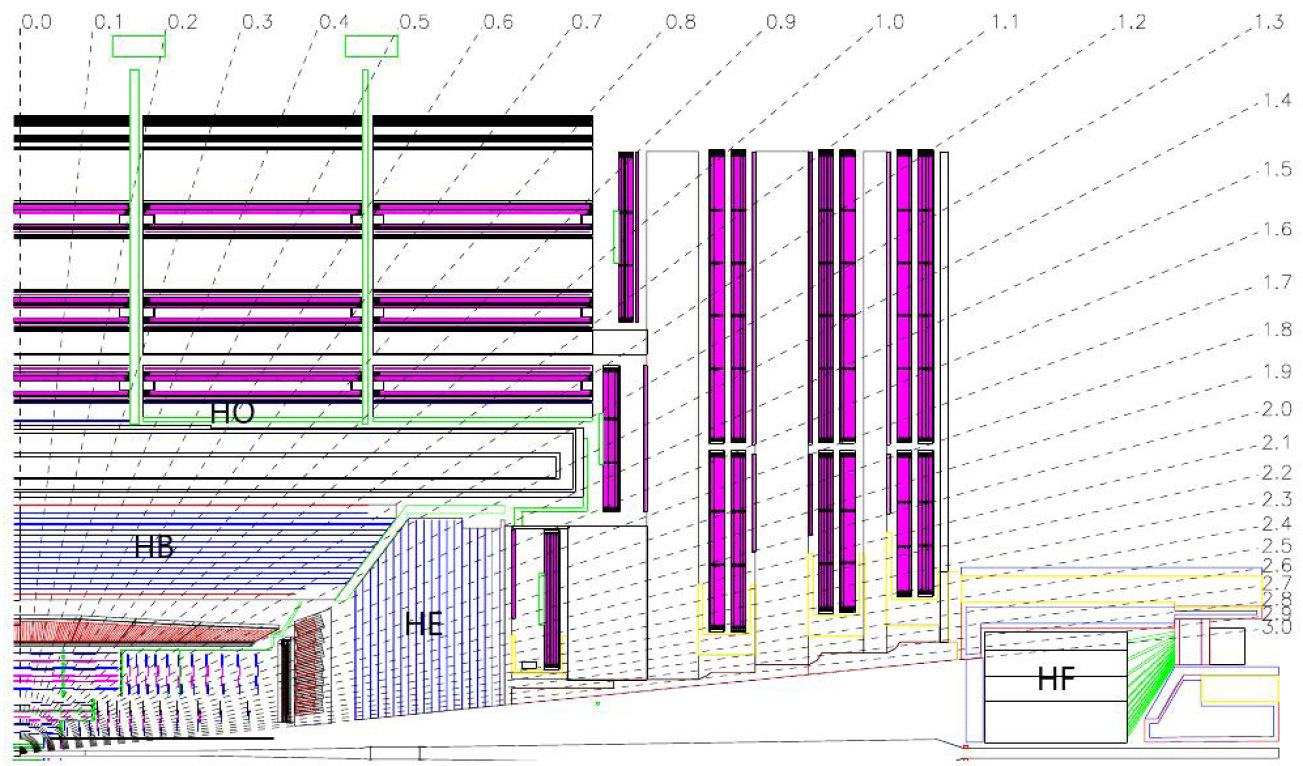
\includegraphics[width=0.9\textwidth]{Figures/detector/cmsHCAL}
  \caption{Longitudinal view of the \ac{CMS} \ac{HCAL}. Locations of the \ac{HB}, \ac{HO}, \ac{HE} and \ac{HF} are shown with values of $\eta$. The purple regions represent the muon detectors which further restrict the volume of the \ac{HO}.
}
  \label{fig:CMShcal}
  \end{center}
\end{figure}

Hadron showers are created in the brass absorber plates, through nuclear interactions in the material, and the plastic scintillator tiles produce blue-violet light when the shower passes through. 
It is read out using wavelength shifting fibres, sending the now green light down transparent fibres to \ac{HPD} which produce an electrical signal proportional to the incident hadron energy.
The first layer of plastic tiles are placed in front of the first absorber plate in order to sample the incoming shower as it develops in the material between the \ac{ECAL} and the \ac{HCAL}.
The final layer of scintillator placed after the final brass plate to catch any late developing showers.
There are 70,000 plastic scintillator tiles in the \ac{HB} and 20,916 tiles in the \ac{HE}.

The \ac{HF} uses a different technology in order to cope with the much harsher environment in which it is situated.
With an average energy of 760~\GeV deposited in the \ac{HF} per pp collision at LHC design energy, peaking at the highest rapidity point closest to the beam line, radiation hardness and occupancy requirements demand alternative materials.
Steel absorber plates are embedded with scintillating quartz fibres, which act to detect the Cherenkov light emitted by charged particles in the shower. 
It is therefore most sensitive to the electromagnetic component of the shower.

The energy resolution of the \ac{HCAL} was measured in pion beam tests. The energy response and 
resolution are shown in Figure~\ref{fig:CMShcalRes}, and the fractional energy response is parametrised
as 
$\frac{\sigma}{E} = \frac{120\%}{\sqrt{E}} \oplus 6.9\%$.

%picture
\begin{figure}[htbp]
  \begin{center}
  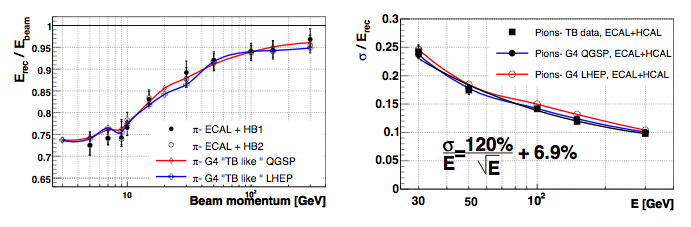
\includegraphics[width=0.9\textwidth]{Figures/detector/HCALres}
  \caption{The raw energy response (left) and fractional energy resolution (right) as a function of energy, for pions, in team beam data.
}
  \label{fig:CMShcalRes}
  \end{center}
\end{figure}

%%%%%%%%%%%%%%%%%%%%%%%%%%%%%%%%%%%%%%%%%%%%%%%%%%%%%%%%%%%%%%%%%%%%%%%%%%%%%%%%%%%%%%%%%%%%%%%

\subsection{The Muon System}
%do i need this
Muons are a powerful tool for recognising signs of interesting physics. 
%Many SUSY models predict excesses of muon decays, for example $B_{s}\rightarrow\mu\mu$, 
%and the Higgs decay $\H \rightarrow \Z\Z$ where both \Z decay to two muons has been called the ``golden plated'' channel.
A relatively easy experimental signature to identify, muons can provide excellent 2- or 4-particle mass resolutions 
as, due to their larger mass, they do not suffer large radiative losses (as electrons do).
%They are therefore of vital importance to the physics programme at \ac{CMS}, such that they take the middle word of the experiment's name.
Muon reconstruction is therefore a central design feature. 
Embedded in the iron flux-return yoke of the solenoid, the muon system combines three methods of gaseous detection to identify, carry out high resolution momentum measurements, and trigger events, up to $|\eta|<2.4$. 
Figure~\ref{fig:CMSmuonSys} shows a cross section of one of the five wheels that make up the barrel section of muon system; there are also two planar endcaps which sit at either end of the detector and enclose it.

%picture
\begin{figure}[htbp]
  \begin{center}
  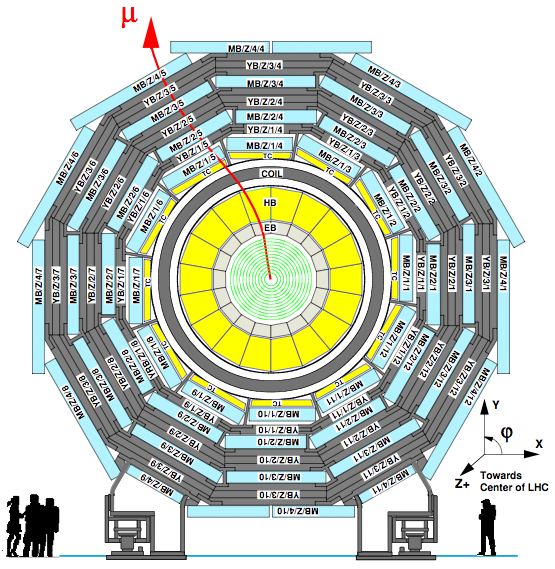
\includegraphics[width=0.7\textwidth]{Figures/detector/muonSystems}
  \caption{One of the 5 wheels of the barrel of the \ac{CMS} muon system. Gaseous detectors are embedded in the iron return yoke of the solenoid; due to the small residual magnetic field in the barrel, \ac{DT}s are used.
}
  \label{fig:CMSmuonSys}
  \end{center}
\end{figure}



In the barrel ($|\eta|<0.9$), magnetic flux is concentrated in the iron return yoke so the residual field is very small.
There is also a low muon rate and neutron induced background, so \ac{DT} chambers are used.
In the endcaps ($0.9<|\eta|<2.4$), magnetic field and muon rate are much higher, so \ac{CSC} are used instead; 
they have a faster response time, higher granularity and better radiation hardness.
Both the \ac{DT} and \ac{CSC} have excellent position resolution.
An additional system of \ac{RPC} in both the barrel and endcaps provide an independent signal which has good time resolution (and poorer position resolution) and serves as a trigger.


By combining information from the tracker, and from either the \ac{DT} or \ac{CSC} and \ac{RPC}, \ac{CMS} has excellent muon reconstruction. 
Precise momentum resolution is achieved for the kinematic range, from 10~\GeV to $>500~\GeV$, shown in  
Figure~\ref{fig:CMSmuonRes}. 

%picture
\begin{figure}[htbp]
  \begin{center}
  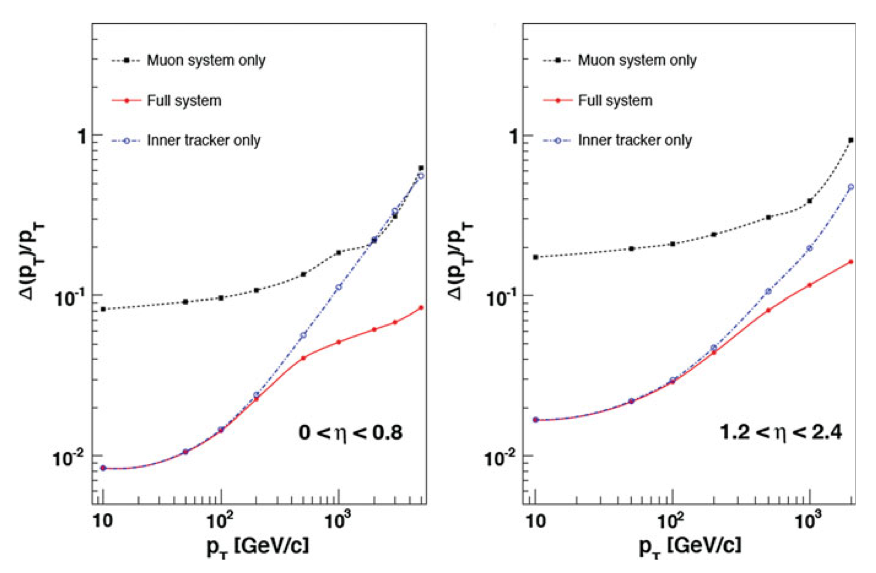
\includegraphics[width=0.8\textwidth]{Figures/detector/CMSmuonRes}
  \caption{Muon transverse momentum resolution, shown as a function of muon \pt in the barrel (left) and the endcaps (right). The resolution of the tracker and muon system is shown, and the enhancement gained by combining the information.
}
  \label{fig:CMSmuonRes}
  \end{center}
\end{figure}

%%%%%%%%%%%%%%%%%%%%%%%%%%%%%%%%%%%%%%%%%%%%%%%%%%%%%%%%%%%%%%%%%%%%%%%%%%%%%%%%%%%%%%%%%%%%%%%
%  ________      ________ _   _ _______   _____  ______ _____ ____  
% |  ____\ \    / /  ____| \ | |__   __| |  __ \|  ____/ ____/ __ \ 
% | |__   \ \  / /| |__  |  \| |  | |    | |__) | |__ | |   | |  | |
% |  __|   \ \/ / |  __| | . ` |  | |    |  _  /|  __|| |   | |  | |
% | |____   \  /  | |____| |\  |  | |    | | \ \| |___| |___| |__| |
% |______|   \/   |______|_| \_|  |_|    |_|  \_\______\_____\____/ 
%                                                                  
%%%%%%%%%%%%%%%%%%%%%%%%%%%%%%%%%%%%%%%%%%%%%%%%%%%%%%%%%%%%%%%%%%%%%%%%%%%%%%%%%%%%%%%%%%%%%%%

\newpage
\section{Event Reconstruction} \label{sec:CMSreco}

It is by piecing together the information from the various subsystems of the \ac{CMS} detector that, for example, a track in the tracking system, or an energy deposit in the \ac{HCAL}, can be attributed to a particle or ``physics object''. 
Figure~\ref{fig:CMSslice} shows a slice of the whole detector with each of the main physics objects traversing it: muons, electrons, photons, and charged and neutral hadrons.
Each of these leaves a different signature.
Charged particles leave tracks in the silicon tracker, curved under the influence of the magnetic field.
Electrons and photons cause electromagnetic showers, leaving energy deposits in the \ac{ECAL}.
Hadrons penetrate further, showering and leaving energy deposits in the \ac{HCAL}. 
Muons are the only visible particles to reach the muon system, where they leave tracks.

%picture
\begin{figure}[htbp]
  \begin{center}
  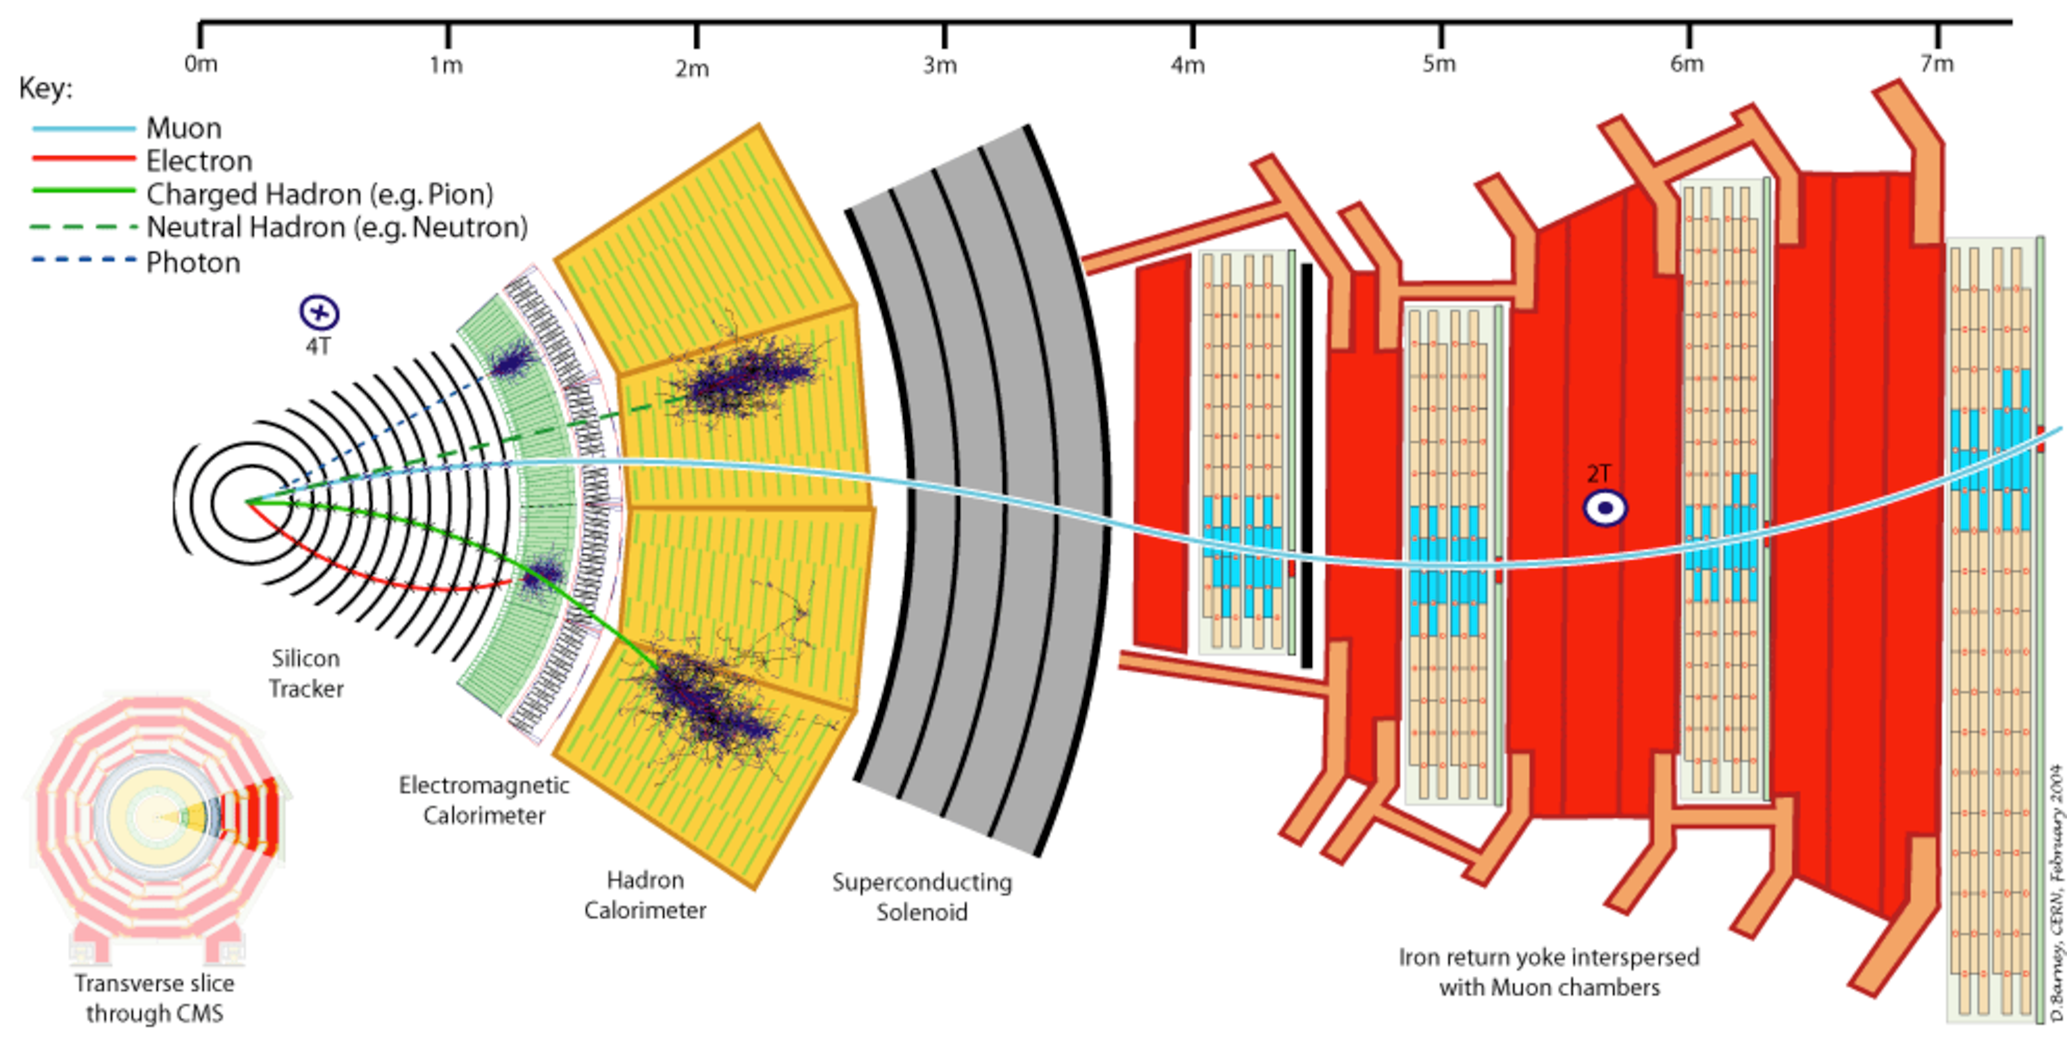
\includegraphics[width=0.9\textwidth]{Figures/detector/CMS_Slice.pdf}
  \caption{A slice of the \ac{CMS} detector is shown, with various particles, or physics objects, traversing it. By combining information from each of the subdetectors, each of the particles produced in an event can be identified and the whole event reconstructed.
}
  \label{fig:CMSslice}
  \end{center}
\end{figure}

Particles can then be identified by combining tracking information with data from the calorimeters and muon system.
If there is an energy deposit in the \ac{ECAL}, the only way to distinguish between a photon or electron is by looking to see if there are hits in the tracker, leading to the position of the electromagnetic shower in the calorimeter. 
Similarly, the momentum measurement of the electron, determined using the curvature of the track it leaves (also used to reconstruct its charge), can be combined with the energy measurement made using the amount of scintillation light produced in the \ac{ECAL} to get a better resolution.
If there is no track leading to the electromagnetic shower, a photon is instead reconstructed.
Hadronic showers in the \ac{HCAL} due to charged and neutral incident hadrons can also be distinguished by their tracks.
A muon will leave the tell-tale sign of hits in the tracker, and hits in the outer muon chambers, where position, momentum and charge measurements from both ensure the initial track in the silicon tracker matches up to the track in the muon system. Dual measurements also lead to enhanced resolution.


Below is a summary of the object reconstruction most relevant to the physics analysis described in Chapter~\ref{chap:sus13009}. 
More information can be found in Ref.~\cite{TDRVOL1}.


\subsection{Jets}
Copious numbers of quarks and gluons are produced during pp collisions in \ac{CMS}, a consequence of the huge \ac{QCD} cross section.
Through the strong interaction they fragment and immediately hadronise, and a spray of hadrons is produced in the direction of an initial quark or gluon.
Various algorithms have been developed in order to group the spray of hadrons into a ``jet'', and assign an energy, direction and transverse momentum to it.

In the analysis presented in this thesis (and in general at \ac{CMS}), the anti-k$_{\mathrm{t}}$ algorithm~\cite{bib:akjets} is used with a distance parameter, $R = 0.5$.
It behaves like an idealised cone algorithm, using a distance parameter to cluster particles into cone shapes, with a radius $R$. Soft particles are clustered with nearby hard particles rather than with themselves, leading to conical jets, which --- crucially --- are resilient to soft radiation on the boundary of the cone.
Likewise, the area of the jet is unaffected by soft radiation on the boundary, and is equal to $\pi R^{2}$. 
These features make the anti-k$_{\mathrm{t}}$ algorithm the preferential jet algorithm at \ac{CMS}, due to its insensitivity to soft radiation that arises from sources such as \ac{PU}; see Figure~\ref{fig:antikT_PU}. 

%picture
\begin{figure}[htbp]
  \begin{center}
  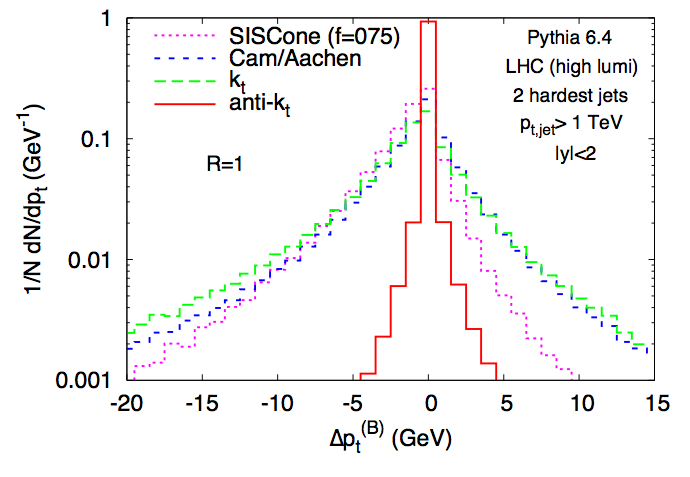
\includegraphics[width=0.7\textwidth]{Figures/detector/PUantiKT}
  \caption{The relative insensitivity of the anti-k$_{\mathrm{t}}$ algorithm to \ac{PU} is shown, compared to other common jet algorithms. The distribution of back reaction, corresponding to the net change in \pt to each of the two hardest jets (where each jet has $\pt>200~\GeV$), when adding \ac{PU}$\sim 25$ to the event, corresponding to \ac{LHC} running conditions in the next phase of data taking starting in 2015. Taken from~\cite{bib:akjets}.}
  \label{fig:antikT_PU}
  \end{center}
\end{figure}

Several types of jets exist at \ac{CMS}, in which the anti-k$_{\mathrm{t}}$ algorithm is given different inputs.
Calorimeter (Calo) jets use information from the calorimeter only.
\ac{ECAL} crystals are grouped in $5\times5$ arrays into ``towers'', which measure $0.087\times0.87$ in $\Delta\phi \times \Delta \eta$ space (in the barrel region) and are matched to aligning blocks of \ac{HCAL}.
The sum of the energy deposits in both layers of calorimeter are used as inputs to the jet algorithm, where towers are treated as massless and an $\eta$ dependent energy threshold has been placed on each tower to reduce the effect of instrumental noise. 

The \ac{PF} algorithm~\cite{PFT-09-001} creates a list of all stable particles in an event: photons, electrons, muons, neutral hadrons and charged hadrons.
Particle momentum, direction and type are determined using all of the subdetectors of \ac{CMS}, 
which, with its silicon tracker, highly granular \ac{ECAL} and strong magnetic field is ideally suited to the task.
The reconstruction of the fundamental constituents of a typical jet --- largely photons, charged hadrons and neutral hadrons --- uses charged particle tracks and calorimeter clusters, termed ``elements''.
A traversing particle is expected to give rise to one, or several elements arising from separate subdetectors. 
%For example, a charged hadron could make one charged particle track and a calorimeter cluster. 
To reconstruct a particle, these elements are therefore grouped into ``blocks'': links of one, two or three elements
that have arisen due to the same object.
Blocks can then be interpreted as individual particles, and the resulting list of reconstructed particle flow particles 
gives a global description of each event.
This list of particles is used as the input to the anti-k$_{\mathrm{t}}$ algorithm, producing \ac{PF} anti-k$_{\mathrm{t}}$ jets.

The energy of a typical jet consists of energy from charged particles (65\%), photons (25\%) and neutral hadrons (10\%).
Therefore, typically, 90\% of the jet energy can be reconstructed with good precision, utilising measurements from the high resolution silicon tracker and \ac{ECAL}. 
Only 10\% of the energy, arising from neutral hadrons, is reconstructed using the relatively poor resolution hadron calorimeter. 
Therefore, \ac{PF} jets, made of reconstructed particles, are much closer to jets made of simulated, \ac{MC} generated particles than those that rely just on calorimeter information alone (such as Calo jets), see Figure~\ref{fig:PFturnOns}.
\ac{PF} jets consequently have excellent position and energy resolution. 
Jet momentum resolution, defined as the ratio $(\pt^{\mathrm{rec}} - \pt^{\mathrm{gen}})/\pt^{\mathrm{gen}}$, (where ``rec'' is for reconstructed, i.e. \ac{PF} or Calo jets, and ``gen'' is for jets taken from simulation) 
is shown in Figure~\ref{fig:PFmomRes}.
It is because of the excellent performance of the \ac{PF} algorithm, as input to the anti-k$_{\mathrm{t}}$ that it is used most commonly across \ac{CMS} analyses, including in the analysis presented in this thesis.

%picture
\begin{figure}[htbp]
  \begin{center}
  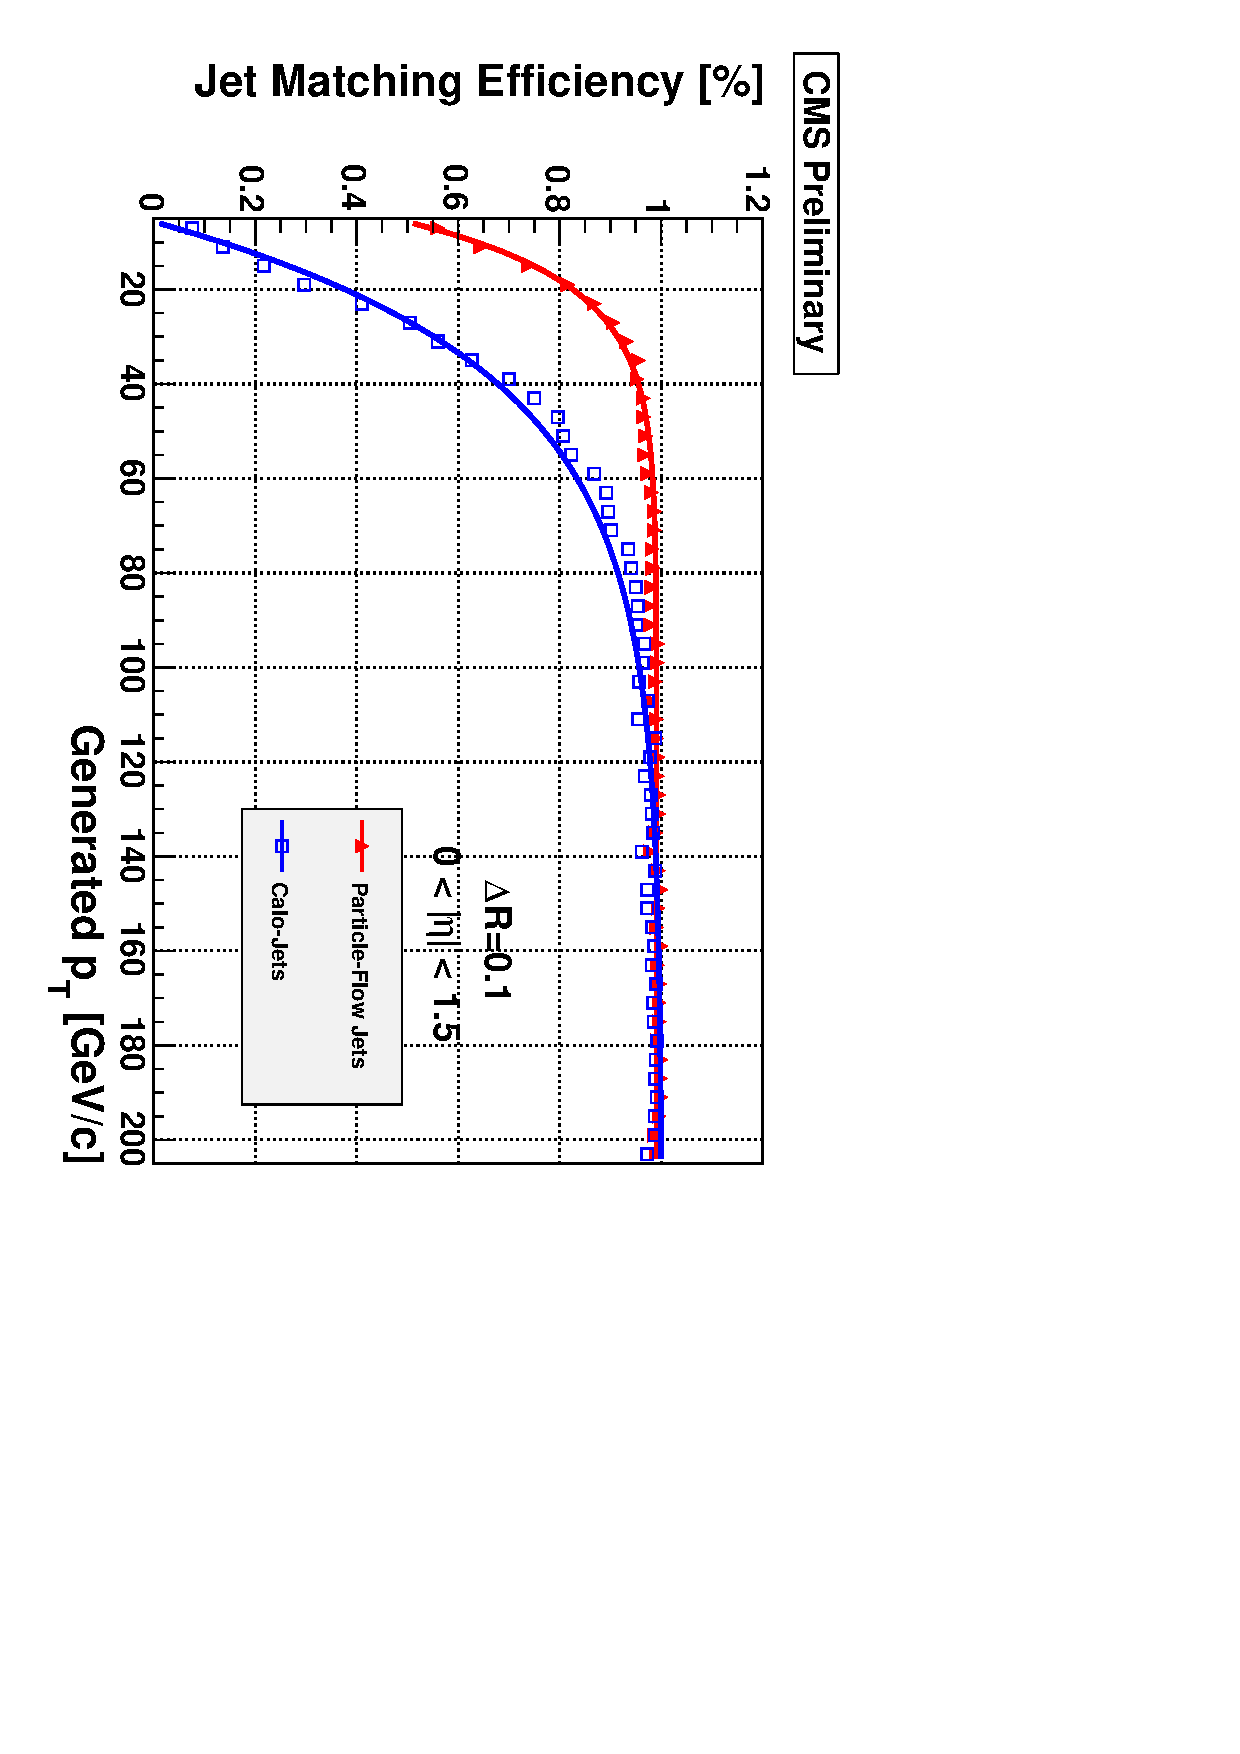
\includegraphics[width=0.33\textwidth, angle =90]{Figures/detector/PFjetvsCalo0p1}
  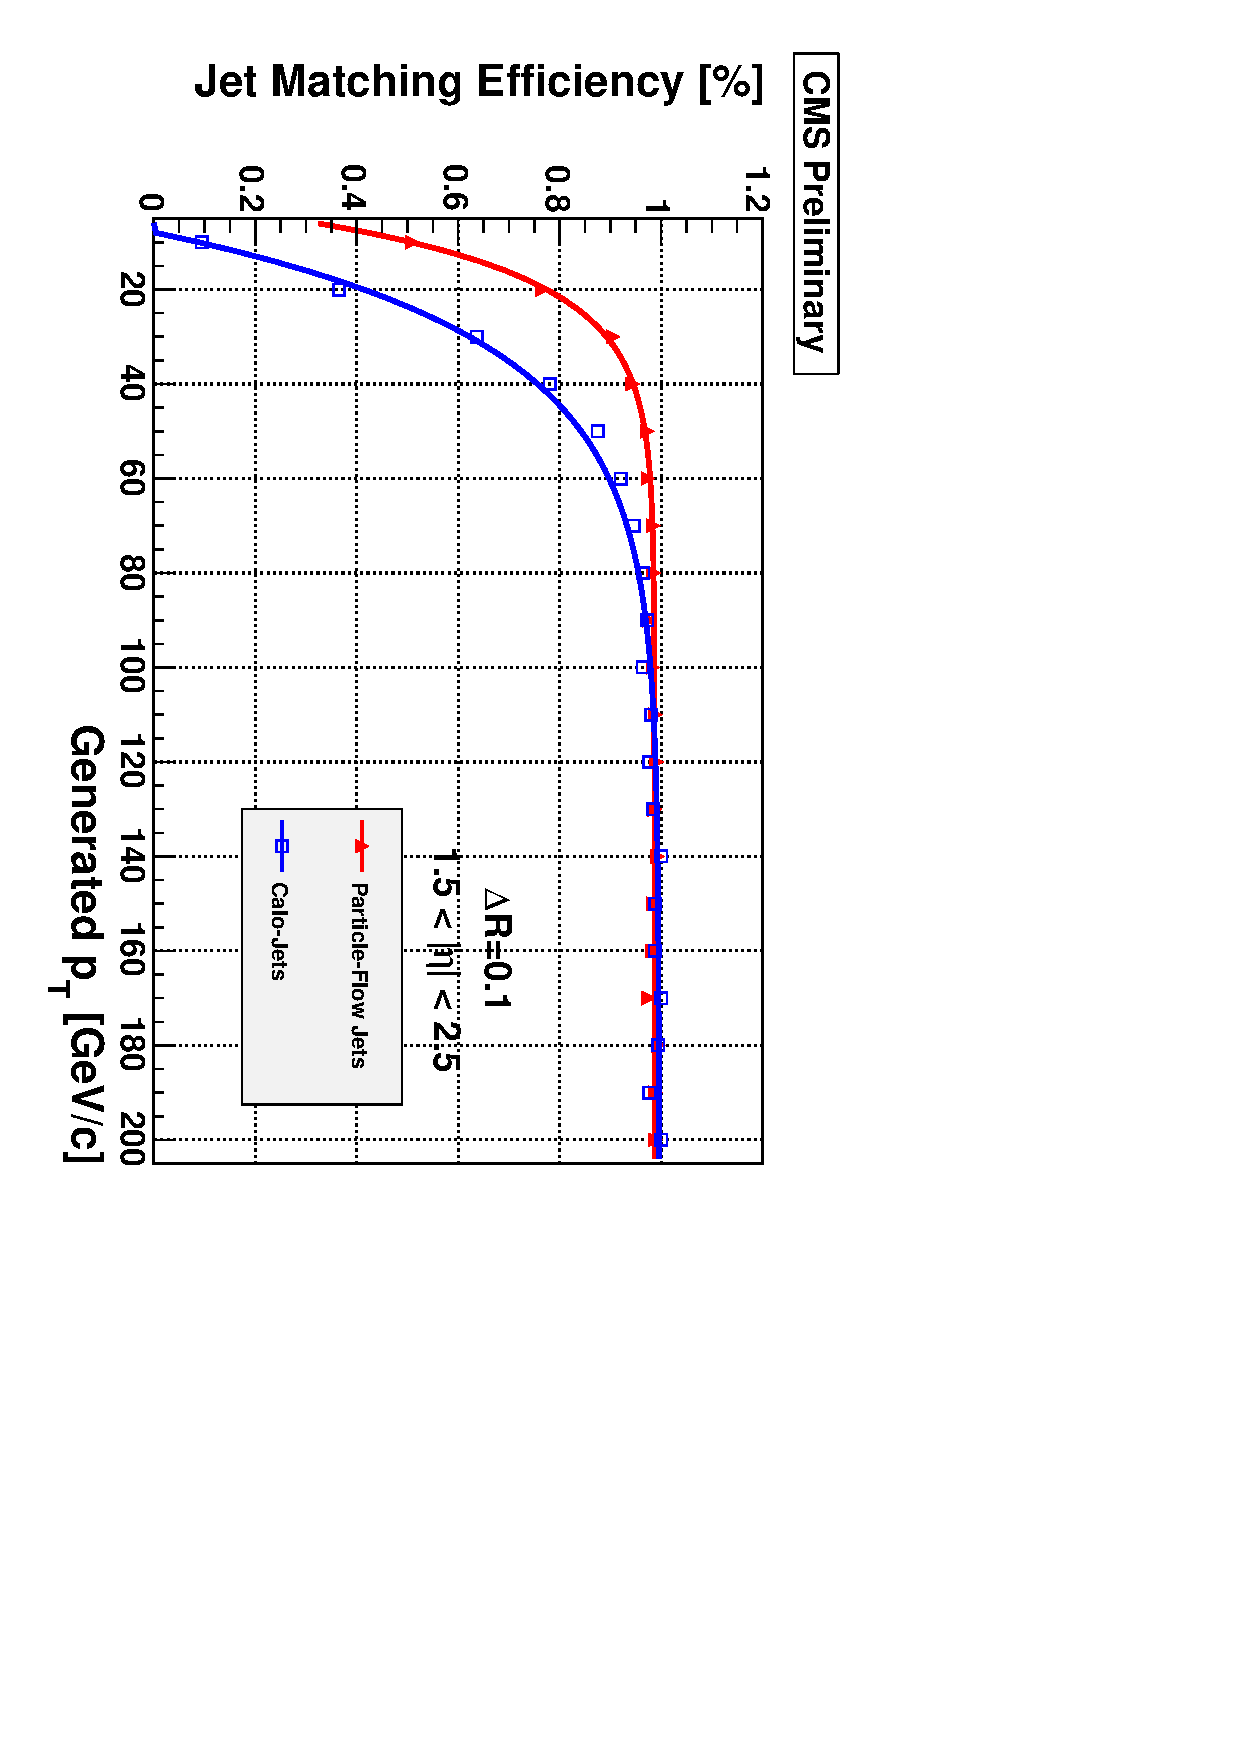
\includegraphics[width=0.33\textwidth, angle =90]{Figures/detector/PFjetvsCalo0p1end}
  \caption{The efficiency of \ac{PF} jets, and Calo jets, matched to generated jets in the barrel region (left) and the endcap (right), taken from~\cite{PFT-09-001}. The superior performance of \ac{PF} jets is evident because they are more efficiently matched to the generator, ``truth'' jets, at a lower \pt threshold: termed a sharper turn-on.}
  \label{fig:PFturnOns}
  \end{center}
\end{figure}

%picture
\begin{figure}[htbp]
  \begin{center}
  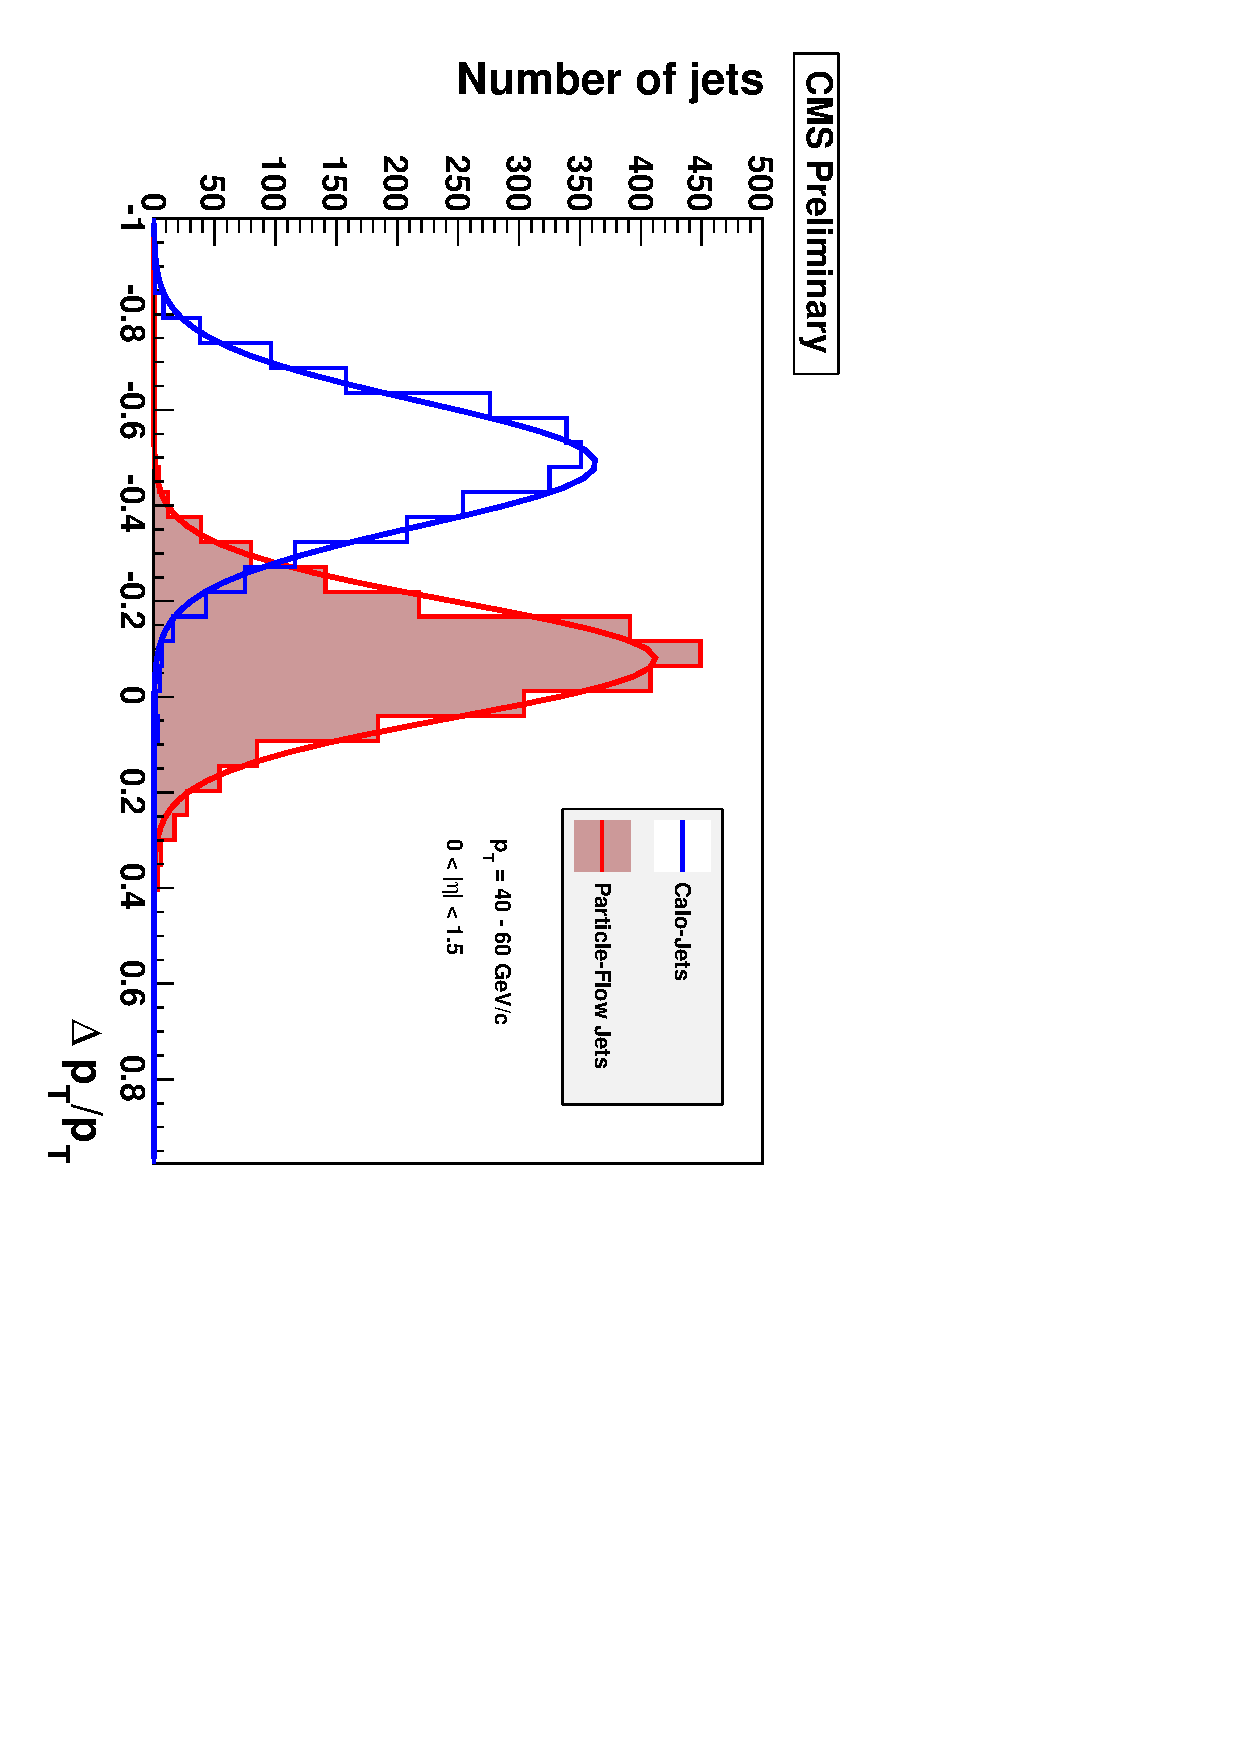
\includegraphics[width=0.33\textwidth, angle =90]{Figures/detector/MomResPFjetCaloJet_lowPt.pdf}
  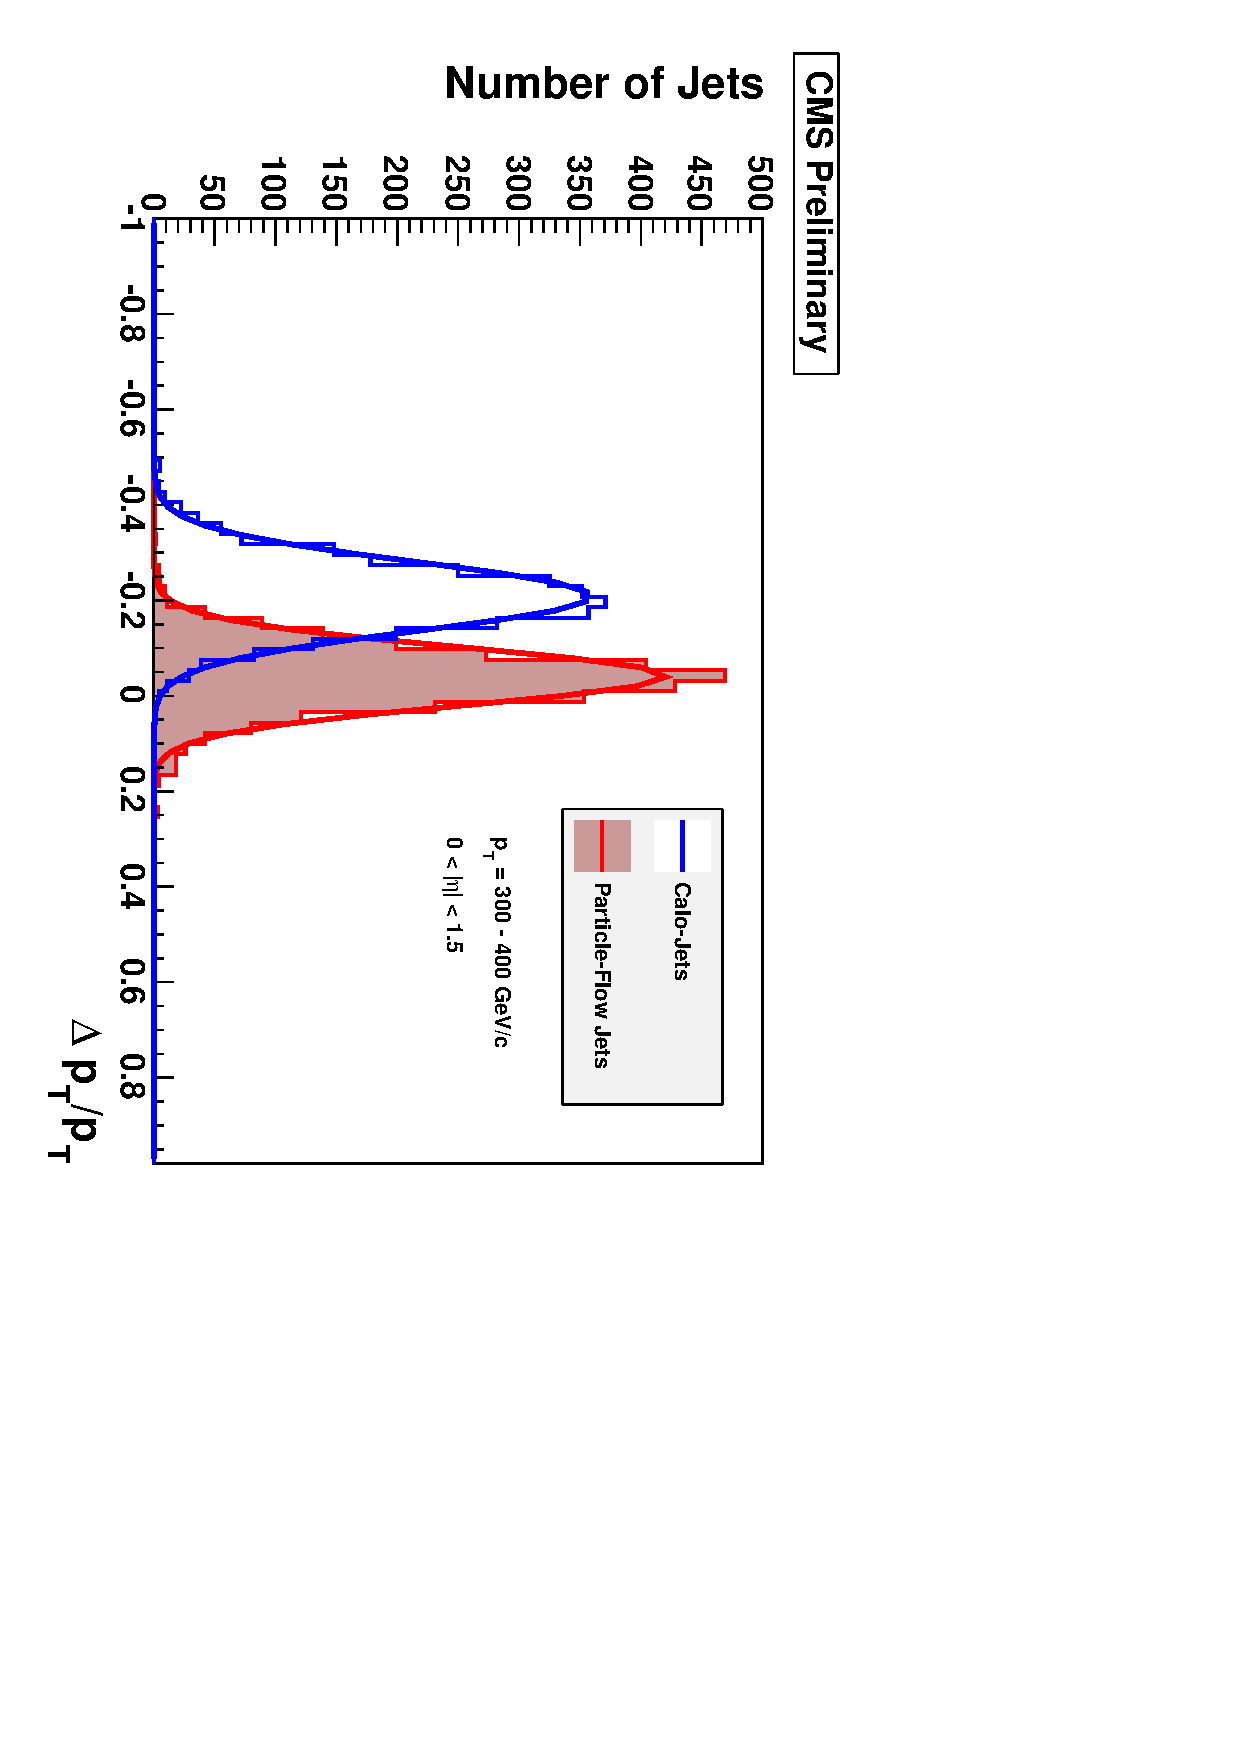
\includegraphics[width=0.33\textwidth, angle =90]{Figures/detector/MomResPFjetCaloJet_highPt.pdf}
  \caption{The momentum resolution, $(\pt^{\mathrm{rec}} - \pt^{\mathrm{gen}})/\pt^{\mathrm{gen}}$ of \ac{PF} jets, and Calo jets, for low energy jets ($40~\GeV<\pt<60~\GeV$) (left) and for high momentum jets ($300~\GeV<\pt<400~\GeV$) (right) in the barrel region, taken from~\cite{PFT-09-001}. Not only are the peaks sharper for \ac{PF} jets, meaning a smaller (and therefore better) overall momentum resolution, but it is also peaking much closer to zero, meaning the jet measurement is much closer to the generated jet momentum.}
  \label{fig:PFmomRes}
  \end{center}
\end{figure}


\subsection{Missing Transverse Energy}

As discussed in the previous sections, \ac{CMS} is nearly hermetic, has coverage up to $|\eta| = 5$ and excellent particle reconstruction; a very complete picture of each event is available. 
As such, is it very well suited to make measurements of weakly interacting particles, such as neutrinos, that do not leave any trace within any subsystem of the detector; and are only evident through an imbalance of transverse momentum.
New physics processes, such as R-parity conserving \ac{SUSY}, would also lead to signatures involving a large imbalance in transverse momentum as the weakly interacting \ac{LSP} exits the detector. \ac{DM} production would also lead to such a signature.
Measurements of missing transverse energy and momentum are therefore crucial to the search for new physics at \ac{CMS}, as they have been crucial in previous discoveries --- for example of the W boson~\cite{bib:Wdiscovery}, and in searches for other processes~\cite{Albajar:173124,Albajar:173125}. 

The missing transverse energy vector, $\METv$ is formed by adding the transverse energy vectors $\sum \ETv$ of all the particles formed in an event. The missing transverse energy vector $\METv = - \sum \ETv$, where $|\METv| = \MET = |\sum \ETv|$; i.e., it is equal in magnitude and opposite in direction to the total visible energy in the event.
In an analogous way to jets (and usually using such jets), $\MET$ can be built using various algorithms. 
Calorimeter (Calo) \MET, in the same way as Calo jets, is built from calorimeter information alone while
\ac{PF} \MET is calculated from all of the transverse energies of reconstructed particles in an event. 
In a similar way to the jet algorithms, a better resolution is achieved using the \ac{PF} algorithm over calorimeter information alone, see Figure~\ref{fig:PFMET}
However, because energy measurements of particle flow objects are driven by calorimeter resolution, particularly for large \ET objects, the improvement is less marked.
In the analysis presented in this thesis, \ac{PF} \MET is used, where any muons present have been removed from the  calculation. It therefore mimics Calo \MET, only with an enhanced resolution. 

%picture
\begin{figure}[htbp]
  \begin{center}
  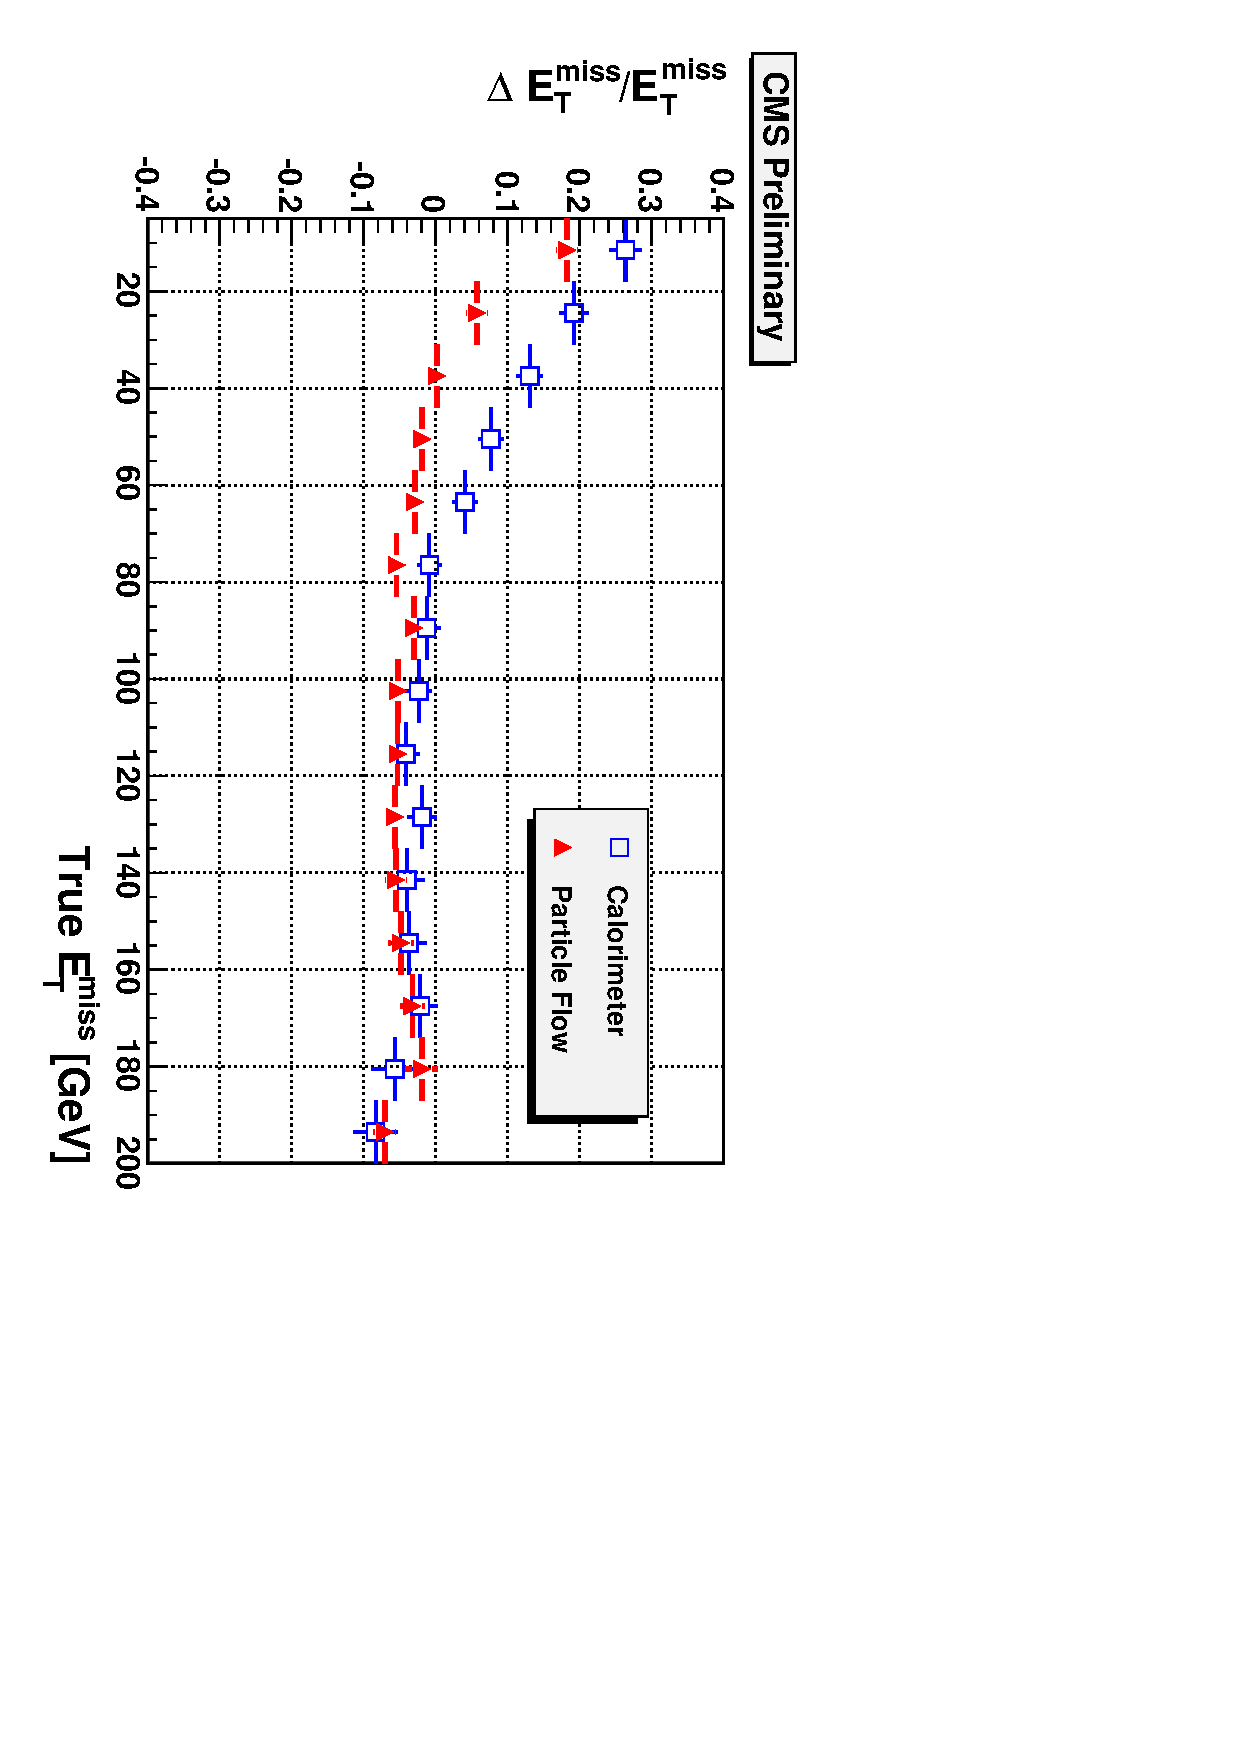
\includegraphics[width=0.53\textwidth, angle =90]{Figures/detector/METresPF.pdf}
  \caption{The momentum resolution, $(E^{\mathrm{miss}}_{T,rec} - E^{\mathrm{miss}}_{T,\mathrm{gen}})/E^{\mathrm{miss}}_{T,\mathrm{gen}}$ of \ac{PF} and Calo \MET, taken from~\cite{PFT-09-001}. An improved resolution is seen using the \ac{PF} algorithm, particularly at low values of \MET. At higher \MET values, energy measurements are dominated by the calorimeter resolution and values using the two different methods converge.}
  \label{fig:PFMET}
  \end{center}
\end{figure}

\subsection{Muons}

Muons are reconstructed using the muon systems and the tracker, and the reconstruction algorithms use the concept of ``regional reconstruction''. 
On the basis of an input or seed from the muon systems, the software only reconstructs the part of the tracker from which the muon causing the seed could originate.
This means that only a very small part (typically a few percent) of the tracker volume must be processed to reconstruct a muon; thereby speeding up the procedure and reducing the CPU power necessary to process an event.

Muon reconstruction has three stages: local, standalone and global reconstruction.
Starting with a seed which defines a region of interest, which could be from the \ac{L1} Trigger seeds (from the \ac{RPC}) or from patterns of hits found in the \ac{CSC} and/or \ac{DT},
a local reconstruction is performed in surrounding compatible muon chambers.
The standalone reconstruction uses information from just the muon system;
measurements of track position, momentum and direction of travel are taken, and extrapolated to the nominal interaction point. 
Global reconstruction then extends the resulting muon trajectories to include hits in the silicon tracker. A track is extrapolated from the innermost muon chamber to the outer tracker surface, and compatible silicon layers determined.
Candidates for the muon trajectory are built from pairs of hits in separate layers of the tracker 
and $\chi^{2}$ of the fit is used to ensure a ``good'' muon candidate; to detect any bremsstrahlung or significant energy loss. 
High energy muons present particular difficulty as they suffer huge energy loss and severe electromagnetic showers in the muon system; the $\chi^{2}$ probability of the fit compared to the the $\chi^{2}$ probability of the tracker only trajectory allows accurate momentum reconstruction of such objects. 

%\subsection{Electrons}

%Electrons (and photons) deposit their energy in the \ac{ECAL} through electromagnetic showers, and approximately 94\% of the energy of an incident electron or photon is contained within a $3\times3$ crystal array.
%Bremsstrahlung and photon conversion in the inner layers of \ac{CMS} lead to an energy spread in $\phi$ under the influence of the magnetic field, which is clustered by building a ``supercluster''~\cite{Cittolin:578006}. 
%Significant energy loss of the incident particle can also occur, depending on the material sitting in front of the \ac{ECAL} at its position, which is taken into account using various $\eta$ reconstruction methods, detailed elsewhere~\cite{Cittolin:578006}.   
%A reconstructed electron is composed of a single track from the interaction vertex matched to a supercluster.





%%%%%%%%%%%%%%%%%%%%%%%%%%%%%%%%%%%%%%%%%%%%%%%%%%%%%%%%%%%%%%%%%%%%%%%%%%%%%%%%%%%%%%%%%%%%%%%
%  _______ _____  _____ _____  _____ ______ _____  
% |__   __|  __ \|_   _/ ____|/ ____|  ____|  __ \ 
%    | |  | |__) | | || |  __| |  __| |__  | |__) |
%    | |  |  _  /  | || | |_ | | |_ |  __| |  _  / 
%    | |  | | \ \ _| || |__| | |__| | |____| | \ \ 
%    |_|  |_|  \_\_____\_____|\_____|______|_|  \_\

%%%%%%%%%%%%%%%%%%%%%%%%%%%%%%%%%%%%%%%%%%%%%%%%%%%%%%%%%%%%%%%%%%%%%%%%%%%%%%%%%%%%%%%%%%%%%%%


\newpage
\section{The Trigger} \label{sec:CMStrig}

%Crucial to the successful operation of \ac{CMS} is the trigger. 
The pp interaction cross section is 100~\mb, while for example, the W boson production cross section is some 6 orders of magnitude less than this, and the rare physics processes that \ac{CMS} was built to search for, such as Higgs boson and \ac{SUSY} production, many times smaller still; see Figure~\ref{fig:ppCrossSec}.
The \ac{LHC} delivers an unprecedentedly high instantaneous luminosity so that such rare physics processes occur, but this also implies that the vast majority of the collisions result in `uninteresting' physics: namely relatively low energy, soft scattering events.
It would be impossible to record the very high volumes of data that come out of \ac{CMS}, some PB s$^{-1}$, and not useful to do so.
Therefore, a very efficient method of recording those events that appear `interesting'
is necessary.% to reduce the 40~\MHz event rate to a more manageable 100~\Hz.
%The two-tier trigger system fulfills this role, via a hardware based online \ac{L1} an software based offline \ac{HLT}.% and is described in Section~\ref{sec:CMStrig}.
%picture

\begin{figure}[htbp]
  \begin{center}
  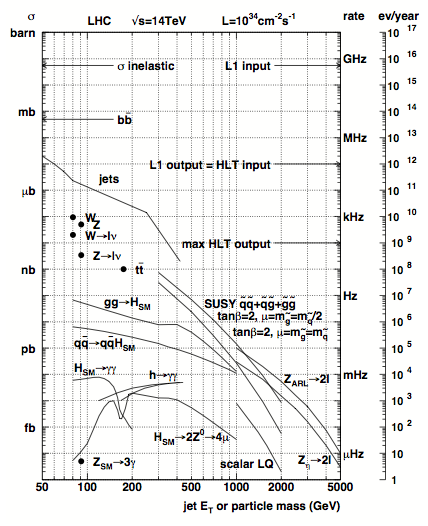
\includegraphics[width=0.49\textwidth]{Figures/detector/ppCrossSections}
  \caption{Inclusive pp cross sections (\sigma) for basic and rarer physics processes, showing some of the phenomena on the physics programme at~\ac{CMS}. Shown on the right are the interaction rates for \ac{LHC} design luminosity, \designLumi. Taken from~\cite{Cittolin:578006}.
}
  \label{fig:ppCrossSec}
  \end{center}
\end{figure}

A two tier trigger system reduces the 40~\MHz \ac{LHC} bunch crossing rate to an output of 100~\Hz, which is then saved offline to be reconstructed ready for physics analysis. 
The hardware based \ac{L1} uses fast algorithms with coarse inputs from the calorimeter and muon system to efficiently select, online (that is at the same rate as \ac{LHC} bunch crossings),
 those events that appear interesting, reducing the 40~\MHz collision rate to 100~\kHz.
A software based \ac{HLT} running on the event filter PC farm at Point 5 takes the output of the \ac{L1} trigger and reduces it further to 100~\Hz, using more sophisticated inputs and algorithms.
Performance of the subdetectors and readiness to collect data, monitored by the \ac{DAQ} system, is supervised by the trigger control system.
Events passing \ac{HLT} selection requirements are sent to the \ac{CERN} Computing Centre where complex algorithms using all the information from the \ac{CMS} detector are used to fully reconstruct the event.
More information on the~\ac{CMS} trigger can be found in Ref.~\cite{Cittolin:578006}.
%%%%%%%%%%%%%%%%%%%%%%%%%%%%%%%%%%%%%%%%%%%%%%%%%%%%%%%%%

\subsection{The L1 Trigger}
Low granularity inputs from the calorimeter and muon system are used to quickly select possibly interesting events, based on predefined and programmable algorithms and criteria.
Parts of the hardware are \ac{FPGA} based, allowing some flexibility in algorithms, while other parts are \ac{ASIC} based, with predefined criteria.
Events are selected if they show signs of interesting physics; for example have jets, electrons/photons, or muons. 
Global quantities such as total transverse energy and total missing transverse energy are also used.  
In order to see if an event contains any of these physics objects above a pre-defined energy threshold or multiplicity, 
the L1 trigger is separated into the Calorimeter Trigger, which looks for jets, photons and electrons, and the Muon Trigger, which looks for muons. 
Global quantities are computed at the \ac{GT} and combined with information from the Calorimeter and Muon triggers, 
and here a decision is made to keep or reject an event.

In the Calorimeter Trigger, information from the \ac{ECAL}, \ac{HCAL} and \ac{HF} are combined.
First, the calorimeter is split into different (geographical) regions, and electron, photon and jet finding algorithms run on the separate parts of the subdetectors at the \ac{RCT}.
Information from the different regions is then combined at the \ac{GCT}.%, where overlaps in the regions are dealt with.
In the Muon Trigger, information from the \ac{DT}, \ac{CSC} and \ac{RPC} are combined.  
Muon track finding algorithms are applied to data from the \ac{DT} and \ac{CSC} at the \ac{RMT},
and the \ac{GMT} combines information from all of the three subdetectors to get an enhanced resolution.
Inputs from the \ac{GCT} and \ac{GMT} are then combined at the \ac{GT}, 
where the decision to keep or discard an event is made.
The architecture of the L1 trigger is shown in Figure~\ref{fig:L1triggerArch}.

There is an inbuilt latency of 3.2~$\mu$s in the \ac{L1} trigger, meaning that on the first bunch crossing, it takes up to 3.2~$\mu$s to transmit the necessary information, and make a decision. 
This is driven by the data storage available for information from the tracker and preshower detectors; 
they need so much data storage that it must be saved before a L1 accept decision, and subsequent event read out, can be made.
The decisions on the rest of the bunch crossings follow at the rate of collisions, and the architecture is ready to accept another event every 25~\ns.


%picture
\begin{figure}[htbp]
  \begin{center}
  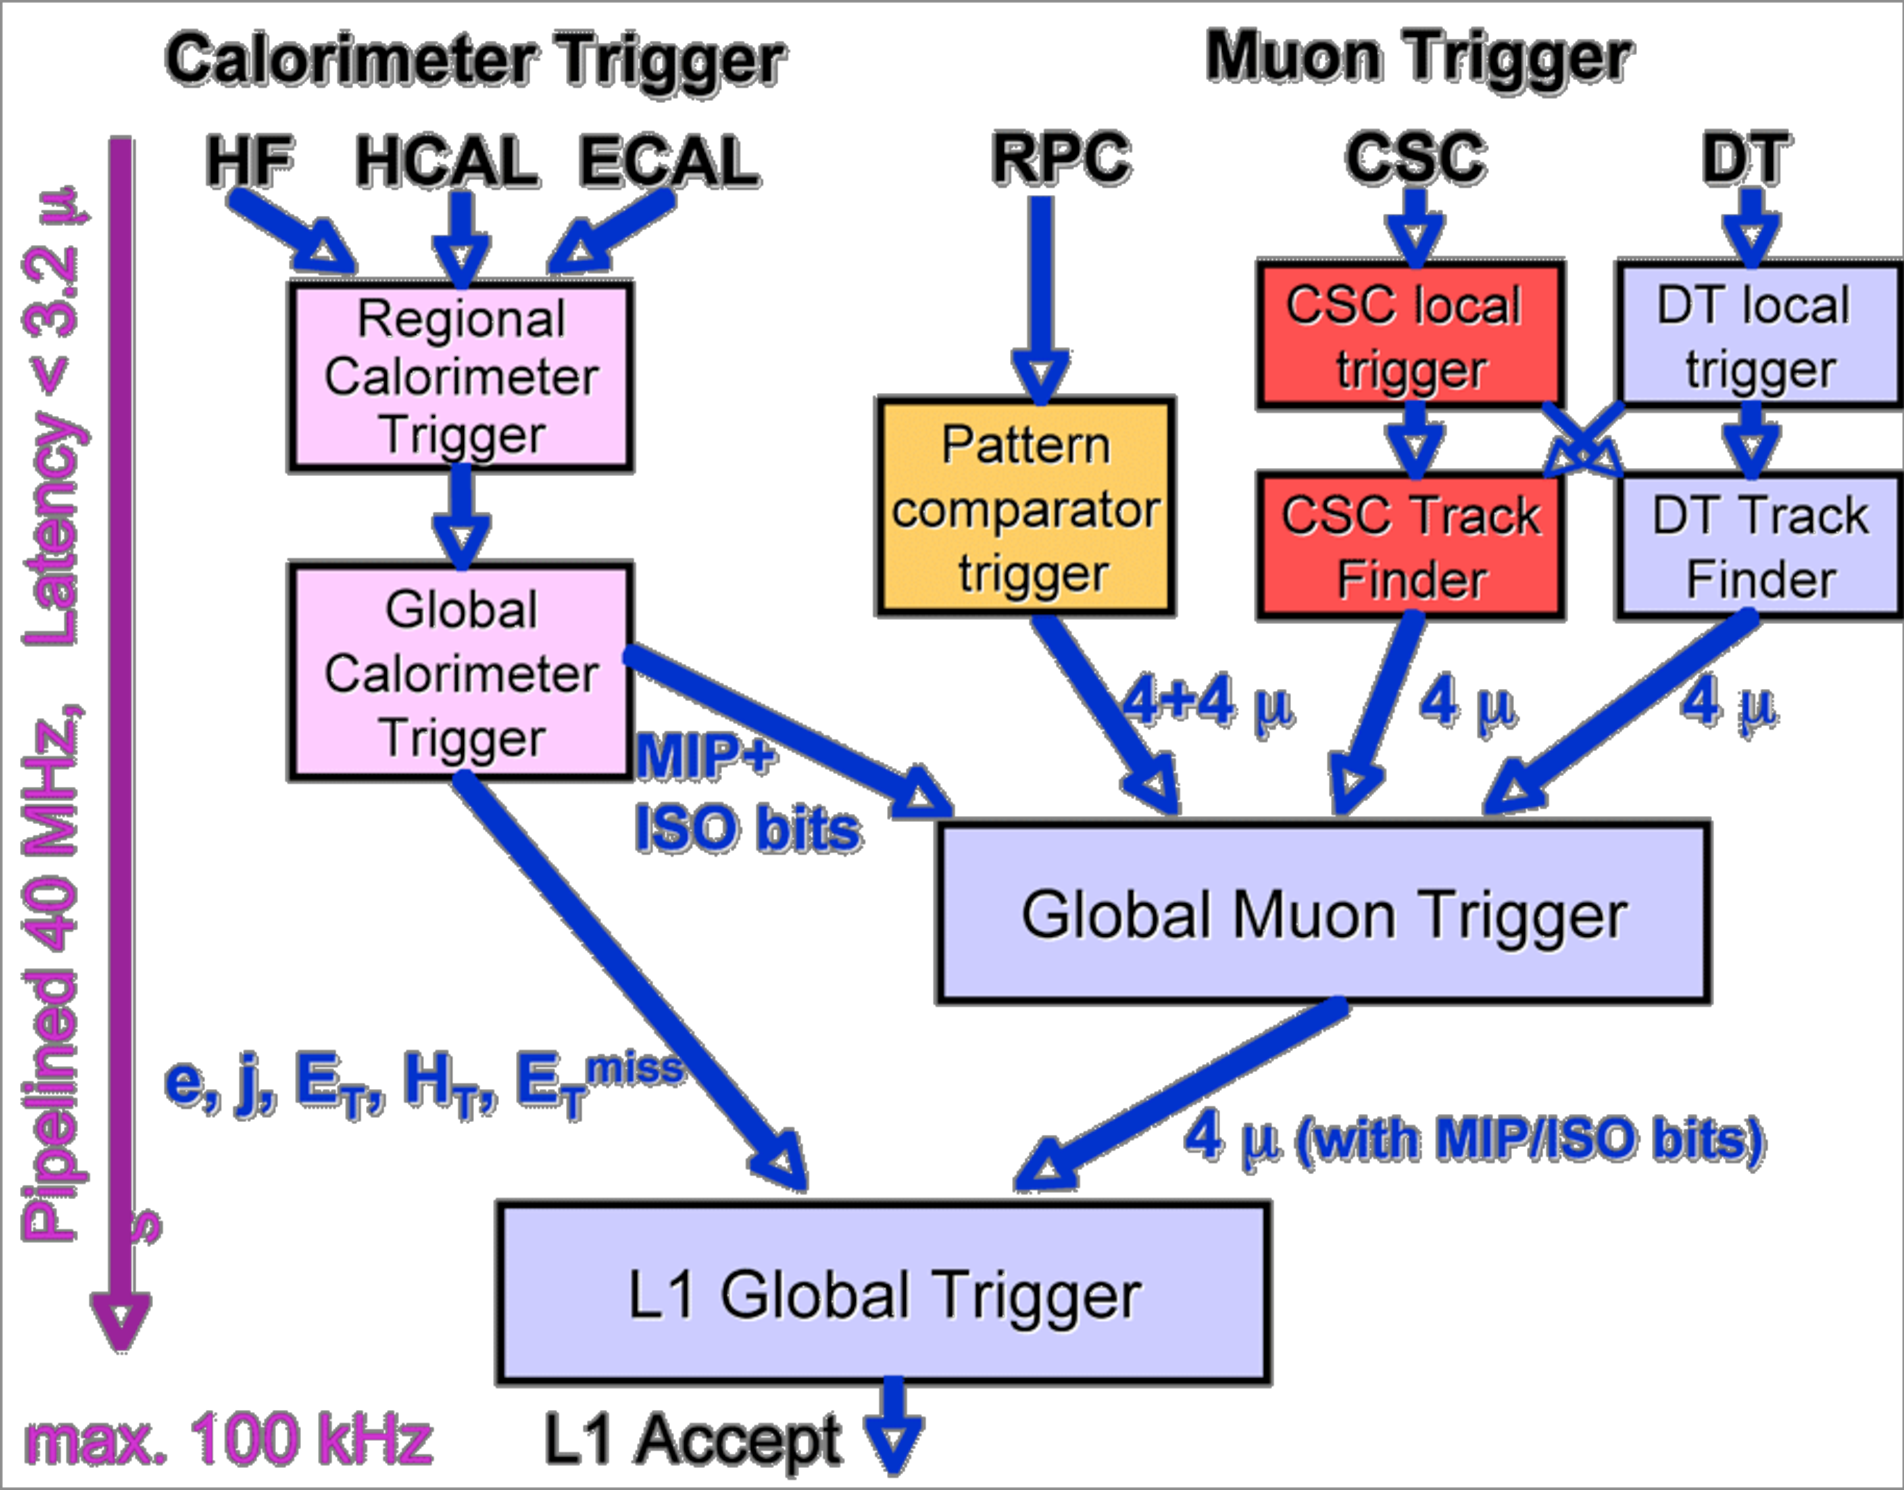
\includegraphics[width=0.6\textwidth]{Figures/detector/L1TriggerArch.pdf}
  \caption{Architecture of the \ac{L1} trigger. The calorimeter trigger takes inputs from the \ac{ECAL}, \ac{HCAL} and \ac{HF}. The muon trigger takes inputs from the \ac{DT}, \ac{CSC} and \ac{RPC}. A decision is made at the L1 \ac{GT}, using inputs from the \ac{GCT} and the \ac{GMT}, of whether to pass an event onto the \ac{HLT} or discard it.
}
  \label{fig:L1triggerArch}
  \end{center}
\end{figure}

A \ac{L1} accept decision is based upon the results of the various physics object reconstruction algorithms.
Typically, every physics analysis has a type of event it is searching for; a particular topology. 
For example, the monojet analysis looks for events with a final state of one high \pt jet and large missing transverse energy. 
At L1, it requires the global variable of an event, total missing transverse energy, above 36, 40 or 50 in \ac{L1} units of energy.
A L1 trigger menu, comprised of all of the required L1 seeds for the whole physics programme at \ac{CMS}, gives a certain bandwidth to each of the seeds. A low threshold seed will typically demand a large amount of bandwidth as more events are likely to be lower in energy, whereas a high threshold will require a lower bandwidth. 
Combined, the output to the \ac{HLT} of all of the L1 seeds in the trigger menu must not exceed the design rate of 100~\kHz.%, limited by the amount of data the \ac{HLT} can process.


\subsection{The High Level Trigger}

When an event is accepted by the L1 trigger, the full detector information for that event (consisting of around 1~MB of data) is passed onto the \ac{HLT}.
On the event filter farm, which consists of over 1000 PC's, all of the detector information for each event is processed.
Information not available at \ac{L1} becomes available. 
The additional computing power and longer time scales mean the full granularity of the calorimeter and tracker information 
(as well as \ac{L1} objects), can be used as inputs to more complex algorithms.
As a result, much more stringent requirements are used to select events of interest, creating datasets which are used for offline analysis.


An analysis will typically use more than one \ac{HLT} trigger, and similarly more than one analysis might use the same trigger (and an event pass more than one trigger).
For example, the monojet analysis %which searches for events which have one high momentum jet and large missing transverse energy,
uses a combination of three triggers which demand large missing transverse energy in every event, or a single high momentum jet in addition to large missing transverse energy.
% The monojet analysis, which searches for events which have one high momentum jet and large missing transverse energy, uses the triggers (or ``paths'')  
% \textsc{\small HLT\_MET120\_HBHENoiseCleaned}
% and
% \newline
% \textsc{\small HLT\_MonoCentralPFJet80\_PFMETnoMu95\_NHEF0p95},
% \newline
% \textsc{\small HLT\_MonoCentralPFJet80\_PFMETnoMu105\_NHEF0p95}.
% The first path requires the missing transverse energy of an event, calculated using calorimeter information only, to be greater than 120~\GeV; in addition, this is quantity is only formed from non-noisy parts of the calorimeter.
% The latter two paths are formed from events which have one jet, reconstructed using the \ac{PF} algorithm~\cite{PFT-09-001}, with transverse momentum above 80~\GeV. Additionally, the missing transverse energy, calculated also with the \ac{PF} algorithm without contributions from muons, must be above 95 or 105~\GeV, and the neutral hadronic energy fraction of the jet must be less than 0.95. 
This allows events with a monojet topology to be selected efficiently; further kinematic and topological selections are applied offline to a dataset formed of events passing these trigger requirements.
Similarly, every physics analysis uses a trigger (or triggers) suited to the topology under investigation.


In the same way that there is a L1 trigger menu, there is also a \ac{HLT} menu 
comprised of all of the \ac{HLT} trigger paths, and the bandwidths they require, which meets the needs of all of the physics analyses at \ac{CMS}.
The total bandwidth of the \ac{HLT} menu must not exceed 100~\Hz or 100 events saved offline per second, limited by the resources necessary to process and store events; namely \ac{CPU}s and disk space available.

